\documentclass[10pt]{article}


% Tous les packages prédéfinis
\usepackage{introLatex}
\usepackage{headfootLatex}
\usepackage{shortcutLatex}
\usepackage{envLatex}
\usepackage{booktabs}
\usepackage{algorithm}
\usepackage{algorithmic}
%\usepackage{algpseudocode}

\graphicspath{{logos/}{figures/}}

\newcommand{\gam}[2]{\ensuremath{\Gamma^{(#1)}_{#2}}}
\newcommand{\gamc}[3]{\ensuremath{\Gamma^{(#1)}_{#2}\[#3\]}}
\newcommand{\gamp}[3]{\ensuremath{\Gamma^{(#1)}_{#2}\(#3\)}}
\newcommand{\gamcf}[3]{\ensuremath{\hat{\Gamma}^{(#1)}_{#2}\[#3\]}}
\newcommand{\gampf}[3]{\ensuremath{\hat{\Gamma}^{(#1)}_{#2}\(#3\)}}

\makeatletter
\def\hlinewd#1{%
\noalign{\ifnum0=`}\fi\hrule \@height #1 %
\futurelet\reserved@a\@xhline}
\makeatother


\usepackage{tikz}
\tikzset { domaine/.style 2 args={domain=#1:#2} }
\definecolor{bleu}{rgb}{0.99,0.69,0.07}

\begin{document}


% Titre du document
\begin{titlepage}
	

\vspace*{-22pt}
\begin{center}

\includegraphics[scale=0.35]{Logo_LPTMC.png}
\hspace*{20pt}

\includegraphics[scale=0.05]{Logo_ENSTA.jpg}
\hspace*{20pt}

\includegraphics[scale=0.10]{Logo_ENSC.jpg}
\hspace*{20pt}

\includegraphics[scale=0.15]{Logo_Versailles.png}
\\
\vspace*{20pt}
\rule{10cm}{1pt}
\vspace*{10pt} \\
\textsc{\textbf{{\large Master 2 de mathématiques : Analyse, Modélisation, Simulation}}\\
 Parcours : Modélisation Simulation}\\
\rule{10cm}{1pt}
\vspace*{20pt} \\
\textbf{\Large Etude numérique des équations \og BMW \fg{} \\ du groupe de renormalisation non perturbatif}\\
\vspace*{10pt}
Gaétan Facchinetti \\
Encadré par : Bertrand Delamotte  et Nicolas Dupuis
{ \\
\vspace*{15pt}
\textit{Laboratoire de Physique Théorique de la Matièe Condensée},\\
\vspace*{5pt}
\textit{Université Paris-Saclay},\textit{Ecole Nationale Supérieure des Techniques Avancées}, \\
\textit{Ecole Normale Supérieure de Cachan}, \textit{Université Versailles Saint Quentin}}\\
\vspace*{20pt}
{\small 27 février - 28 juillet 2017 }

\end{center}


\vfill
\hfill

\includegraphics[scale=0.25]{parisSaclay.jpg}
\pagebreak

%\vspace*{4pt}
\end{titlepage}
\pagebreak

\strut
 \thispagestyle{empty}
\newpage






% On commence le compteur de page ici
 \setcounter{page}{1}

\begin{flushleft}
\color{bleu}
{\fontsize{14}{14} \selectfont
	\textbf{Remerciement}}\\

\color{black}
\end{flushleft}
Je souhaiterais remercier l'ensemble des membres du LPTMC que j'ai eu le plaisir de rencontrer pour leur accueil chaleureux et leur aide tout au long de mon stage. Je souhaiterais tout particulièrement remercier Bertrand Delamotte et Nicolas Dupuis qui m'ont 




\begin{flushleft}
\color{bleu}
{\fontsize{14}{14} \selectfont
	\textbf{Acknowledgments}}\\

\color{black}
\end{flushleft}
I would like to thank all the members of LPTMC whom I had the pleasure to meet for their warm welcome and their help. I would particulary like to thank Pr. Janne Ruostekoski who has helped and guided my with the project as well as the administrative procedures.
\vspace*{11pt}



\begin{center}
\rule{13.7cm}{.5pt}
\end{center}

\vspace*{-11pt}
\begin{abstract}
Nous montrons qu'un ensemble d'atomes froids isotropes dans un réseau optiques 2D peut permettre de stocker de la lumière sur des temps sous-radiant à l'aide d’interactions dipolaires collectives. Nous excitons les dipôles atomiques dans le plan du réseau par une lumière plane monochromatique proche résonance puis en manipulant correctement les niveaux d'énergie atomiques par effet Zeeman nous avons réussi à tourner les y rendre perpendiculaire. En réalisant un traitement exact sur des réseaux réalistes nous obtenons des temps d'émission spontané collectifs d'environ huit fois le temps d’émission spontané d'un atome unique. Nous montrons aussi que les distances interatomiques et la taille du réseau jouent un rôle important pour augmenter ce temps ; un total de 400 atomes étant suffisant pour obtenir la sous-radiance annoncée. De plus il serait très avantageux de parvenir à créer des réseaux avec un meilleur confinement des atomes puisque pour un confinement parfait nous obtenons un stockage cent fois plus long qu'avec un atome unique. Enfin l'étude de la transmission de la lumière diffusée met en avant les résonances du système ainsi que la possibilité de l'utiliser comme détecteur de champ magnétique. 
\end{abstract}

\begin{center}
\rule{8cm}{.5pt}
\end{center}


\renewcommand{\abstractname}{Abstract}
\begin{abstract}
We show that an atomic ensemble of colf atom in a 2D lattice can be used to store light on subradiant times thanks to dipole-dipole collective interactions. We exite dipole moments in the plane of the lattice with a near resonant plane monochromatic weak light and accurately handling the atomic levels with Zeeman effect we manage to spin them to be oriented perpendicularly and trap the photons. We realized an exact treatment with realistic lattices parameters and found a collective linewidth up to eight times less the linewidth of a single atom. We show that the lattice-spacing and the number of atoms has a important impact on that collective linewidth and a that a lattice of 400 atoms is large enough to reach the previous subradiance. Moreover it would be beneficial to create lattice confinment of the atomes even stronger that what is experimentally currently possible since a perfect confinement gives linewidths greater that one hendred times the linewidth of a single atom. Eventually the study of the transmission showed the system resonances and the possibility to use it as a weak magnetic field detector.  
\end{abstract}


\begin{center}
\rule{13.7cm}{.5pt}
\end{center}

\pagebreak 

\tableofcontents

\pagebreak
\begin{multicols}{2}

\section{Introduction}

La physique statistique établit un cadre permettant de calculer les grandeurs macroscopiques, dites aussi thermodynamiques, des problèmes mettant en jeu des systèmes avec un très grand nombre de degrés de degré de libertés en interaction. Pour donner une image de ce que cela signifie, on considère un litre d'eau enfermée dans une boite. Ce litre d'eau est constitué de $\sim 10^{24}$ molécules qui peuvent vibrer, se déplacer ou tourner dans les trois directions de l'espace et avec une certaine vitesse. La position d'une seule de ces molécules représente trois degrés de libertés (puisque l'on est en 3 dimensions) du système total, son orientation, ou sa vitesse aussi, etc. On remarque alors que l'on obtient, pour une seule môle, un nombre gigantesque de degrés de libertés qui peuvent interagir ensembles (ici par l'intermédiaire, entre autre, des collisions des molécules, de l'attraction gravitationnelle ou des interactions électromagnétiques). Il n'est donc pas possible de déterminer les propriétés physiques macroscopiques de ce système en étudiant un à un la dynamique des degrés de libertés le constituant, ce pourquoi on a recours aux statistiques. 

Nous allons nous intéresser ici plus particulièrement à un domaine particulier de la physique statistique et de la thermodynamique qu'est l'étude des transitions de phase. Pour cela commençons par décrire ce dont il s'agit, puis nous expliciterons ce que que nous allons y étudier. \\


\subsection{Transitions de phases}

En thermodynamique on appelle phase un milieu possédant des propriétés physiques et chimiques macroscopiques homogènes. Or, avec la modification de certains paramètres (comme la température, la pression, etc.), un système peut changer de phase ; il se produit alors une transition de phase. Landau a classé ces transitions suivant deux types : celles du premier ordre et celles du second \cite{toledano1987landau}. Cette classification se fonde sur la continuité ou non de certaines fonctions thermodynamiques au moment de la transition. 
Le passage de l'eau de l'état liquide à l'état gazeux par modification de la température à pression constante est un bon exemple \cite{} de transition du premier ordre. La perte du caractère aimanté d'un métal lorsqu'on le chauffe au dessus d'une certaine température à pression constante, correspond, en revanche, à une transition de phase du second ordre \cite{kochmanski2013curie}. On s'intéresse plus particulièrement ici aux phénomènes physiques particuliers qui se produisent lors des transitions du second ordre. \\

Pour comprendre quels sont ces phénomènes considérons (comme dans toute la suite de cette étude) un système que l'on peut faire changer de phase en imposant sa température $T$. On appelle $T_c$, température critique, la température à laquelle se produit la transition. Il est alors possible de définir sur ce système une fonction de corrélation $G^{(2)}(r)$ qui décrit quantitativement l'influence que deux degrés de libertés du système séparés d'une distance $r$ ont l'un sur l'autre. Notons bien que plus la distance entre les deux sera grande moins cette influence sera forte et donc plus la fonction de corrélation sera faible. A cette fonction, qu'il est possible de déterminer expérimentalement \cite{Bellac2012}, on y associe une longueur $\xi$ qui définit approximativement la distance à partir de laquelle deux degrés de libertés du systèmes n'ont plus d'influence l'un sur l'autre.\\

On observe expérimentalement qu'au moment d'une transition de phase du second ordre, pour $|T-T_c| \rightarrow 0$, à la fois $\xi$ et $G^{(2)}$ divergent, selon les lois 
\begin{equation}
	\xi \sim |T-T_c|^{-\nu} 	\quad \text{et} \quad G^{(2)}(r) \sim |r|^{2-d-\eta},
\end{equation}
où $d$ est la dimension physique du système et $\nu$ et $\eta$ sont deux réels positifs appelés les \emph{exposants critiques}. Notons qu'il existe aussi comme cela plusieurs autres grandeurs desquelles ont peut extraire différents exposants critiques. Le point essentiel étant que tous les systèmes ayant les mêmes propriétés de symétries possèdent les mêmes exposants critiques, on dit qu'ils appartiennent à la même classe d'universalité.\\


\subsection{Intérêt du groupe de renormalisation et des équations BMW}

Le groupe de renormalisation (RG) permet de montrer l'effet d'universalité sur les exposants critiques et de les calculer. L'approche par le RG a permis d'obtenir déjà d'excellents résultats \cite{} pour différents systèmes étudiés comparé aux expériences et autres méthodes comme les simulations Monte-Carlo. Cependant elle reste limitée dans ces applications car elle se fonde sur des approximations de "théorie des perturbations" pour pouvoir mener les calculs qui ne permettent de ne calculer par exemple que les exposants universels critiques mais pas les grandeurs non universelles comme la température critique.\\

Le groupe de renormalisation non perturbatif (NPRG) permet de répondre à ce problème en reprenant le principe du RG sous une approche différente permettant d'accéder à des équations exactes. Cependant, en pratique, ces équations ne sont pas solubles et il faut faire d'autres approximations, comme l'approximation BMW, pouvant être d'autre nature que celle de la théorie des perturbation pour pouvoir récupérer à la fois les exposants critiques et les grandeurs non universelles, bien que cela reste compliqué en pratique. \\

Dans cette étude nous avons repris une simulation d'équations intégro-différentielles non linéaires obtenues par l'approximation BMW pour des systèmes régis par une certaine symétrie \cite{LeonardThesis}. Elle  a déjà permis de déterminer des exposants critiques avec précision pour certains systèmes mais elle présente des comportements étranges et instables pour d'autres. Le but était donc de rechercher quelles en étaient les causes et essayer de résoudre les problèmes. En outre nous avons aussi réaliser la simulation des équations BMW pour un autre modèle afin d'essayer d'en récupérer la température critique.  \\

Dans une première partie nous rappelons les origines du modèle du RG et du NPRG puis nous l'utilisons pour expliquer la structure des équations BMW dans le cas de systèmes possédant une symétrie dite $O(N)$ et étudier numériquement leur résolution et la recherche des exposants critiques associés. Ensuite nous appliquerons le modèle BMW au système d'Ising en deux dimensions afin de tester s'il permet de retrouver la température et les exposants critiques que l'on connait par la résolution analytique faite par Onsager \cite{Onsager}. 


\vspace*{11pt}



\section{Origine du modèle}
\subsection{Un peu de thermodynamique et de physique statistique}

Nous résumons dans cette sections quelques concepts fondamentaux de la thermodynamique et de la physique statistique \cite{diu2007thermodynamique} nécessaires à l'introduction du groupe de renormalisation. \\

Considérons un système à $P$ corps dans un ouvert à $d$ dimensions $\Omega$ de volume $|\Omega|$. On considère que l'ensemble des $N$ degrés de liberté de chacun de ces $P$ corps peuvent être décrit suivant leur position $\rv$ grâce à un ensemble de vecteurs $\{{\varphiv_\rv}\}_\rv$. Le vecteur $\varphiv_\rv$ possède $N$ composantes représentant chacune la valeur d'un degré de liberté du corps situé en $\rv$. Cependant comme nous en avons déjà discuté, nous étudions des systèmes macroscopique, ou autrement dit, des systèmes dans la limite thermodynamique où le nombre $P$ de corps est très élevé. Suffisamment élevé pour considérer que l'ensemble de valeurs ${\{{\varphiv_\rv}\}}_\rv$ discrètes peut en réalité s'exprimer comme une fonction $\varphiv : \rv \in \Omega \rightarrow \varphiv(\rv) \in \R^N$, telle que $\varphiv \in \( \Cc^{\infty}(\Omega)\)^N$. Ceci s'appelle le modèle continu. \\

La dynamique du système est alors régie par un une fonctionnelle de $\varphiv$ : l'hamiltonien $H[\varphiv]$. Avec le formalisme canonique de la physique statistique \cite{rohtuA} nous savons que nous pouvons connaitre toutes l'information sur les propriétés macroscopiques du système en étudiant sa fonction de partition $\Zc$ définie par l'expression 
\begin{equation}
\Zc \equiv \int \Dc \varphiv \, \exp\left\{- H[\varphiv]\right\}, 
\end{equation} 
Cette intégrale est une intégrale fonctionnelle \cite{} sur l'ensemble des champs $\varphiv$ permis par le système (i.e. une somme continue sur l'ensemble des configurations possibles des $P\times N$ degrés de liberté du système). Cependant elle ne peut pas être, de manière générale, calculée pour un $H$ quelconque.\\

Considérons l'hypothèse physique selon laquelle $H$ peut se décomposer en deux parties distinctes,
\begin{equation}
H[\varphiv] = S[\varphiv] - \int_{\Omega} \hv \varphiv,
\end{equation} 
où $S$ est appelée l'action du système (il s'agit en fait de l'hamiltonien du système isolé) et le deuxième terme correspond à l'excitation du système par un champ $\hv$ extérieur. Ainsi $\Zc$ devient une fonctionnelle de $\hv$ et nous définissons l'énergie libre du système comme étant 
\begin{equation}
  W[\hv] = \text{ln}{\(\Zc[\hv]\)}
\end{equation}
En utilisant la notion de dérivée fonctionnelle nous pouvons alors introduire le tenseur des fonctions de corrélations à $n \in \bbrac{1,N}$ corps. Ces fonctions sont très importantes car, comme mentionné dans l'introduction, c'est celle à deux corps qui nous permet de déterminer les exposants critiques $\nu$ et $\eta$. Pour $j \in \bbrac{1,n}$, on pose $\{i_j\} \subset \bbrac{1,N}$ avec $\text{card}(\{i_j\}) = j$. 
\begin{equation}
  G^{(n)}_{\{i_j\}} [\{\rv_{j}\} ; \hv] = \derd{^n W[\hv]}{h_{i_1}(\rv_1) ... \delta h_{i_n}(\rv_n)}
\end{equation}
Cependant ces grandeurs ne peuvent pas se calculer directement. Or, comme l'énergie libre est une fonction convexe \cite{diu2007thermodynamique} on peut définir, une grandeur que l'on parviendra à calculer, le potentiel Gibbs qui est une fonctionnelle du champ $\hv$ définie par transformation de Legendre selon 
\begin{equation}
  \Gamma [\phiv] = - W[\hv] + \int_{\Omega} \hv \phiv,
\end{equation}
Avec, en notant $\left< ... \right>$ la moyenne statistique,
\begin{equation}
  \phiv[\rv, \hv] = \left< \varphiv(\rv) \right> = \derd{W[\hv]}{\hv(\rv)}
\end{equation}
\begin{equation}
  \left< \varphiv(\rv) \right> = \frac{1}{\Zc} \int \Dc \varphiv \, \varphiv(\rv) \exp\left\{- H[\varphiv]\right\}, 
\end{equation}
On introduit aussi une notation pour les tenseurs de dérivées fonctionnelles de $\Gamma$ avec 
\begin{equation}
  \Gamma^{(n)}_{\{i_j\}} [\{\xv_{j}\} ; \phiv] = \derd{^n \Gamma[\phiv]}{\phi_{i_1}(\xv_1) ... \delta \phi_{i_n}(\xv_n)}
\end{equation}
On montre alors \cite{Delamotte2012}, qu'au sens d'inverse d'opérateur, comme définie en annexe,
\begin{equation}
  G^{(2)}_{i_1 i_2}[\hv] = \(\Gamma^{(2)}_{i_1 i_2}[\phiv]\)^{-1}  
\end{equation}

Il faut donc retenir que la connaissance du potentiel de Gibbs équivaut à la connaissance de la fonction de corrélation à deux points et elle nous permet alors aussi de retrouver les exposants critiques qui nous intéressent. \\

En outre la connaissance de $\Gamma[\phiv]$ a aussi un autre avantage important puisqu'il correspond, lorsque $\phiv$ est uniforme, à un facteur de volume $|\Omega|$ près, au potentiel du système que l'on note $V$ selon :
\begin{equation}
	V(\phiv) = \frac{1}{|\Omega|}{\left. \Gamma[\phiv] \right|}_{\phiv \text{ unif.}},
\end{equation}
Et ce sont la position du minimum global de $V$ noté $\phiv_0$ qui nous informe sur la nature de la phase dans laquelle se trouve le système. Si jamais $\phiv_0 \neq 0$ alors la température du système est inférieure à la température critique : on dit qu'il est dans la phase basse température. En revanche si  $\phiv_0 = 0$ la température est au dessus de la température critique et le système est dans la phase haute température.\\
\begin{figure}[H]
\begin{center}
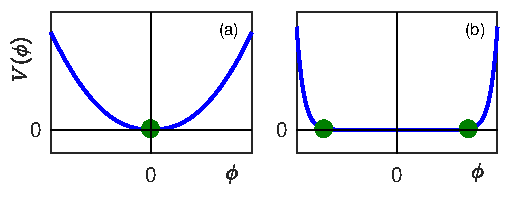
\includegraphics[width=0.95\columnwidth]{CourbePot1.pdf}
\caption{Allure du potentiel pour un champ n'ayant qu'une seule composante : $\phiv = \phi$. La position de $\phi_0$ est symbolisée par les points verts. Dans le cas (a), nous sommes dans la phase dite haute température. Dans le cas (b) le potentiel est toujours une fonction convexe mais elle est extra plate autour de l'origine. En physique on dira que le minimum de V ne se trouve pas vraiment en $0$ mais sur les bords de la région plate, suivant certains critères. Remarquons qu'il s'agit bien alors de fonctions concaves et paires.}
\end{center}
\end{figure}
\vspace*{-11pt}
Développons à présent les théories du RG et du NPRG qui partent des quelques formules rappelées ici. 



\vspace*{11pt}
\subsection{Le groupe de renormalisation (RG)}


\subsubsection{Transformée de Fourier}

Nous rappelons ici de manière synthétiques les principales idées du RG développé par Wilson \cite{wilson}. Commençons pour cela par définir la transformée de Fourier du champ $\varphiv$ appartenant à $L^2(\Omega)$ par 
\begin{equation}
\begin{split}
\hat{\varphiv}_\pv = \frac{1}{\sqrt{|\Omega|}}\int_\Omega \varphiv(\rv) \, e^{-i \pv . \rv} \dd \, \rv, \\
\varphiv(\rv) = \frac{1}{\sqrt{|\Omega|}}\sum_\pv \hat{\varphiv}_\pv \, e^{i \pv  .\rv}
\end{split} 	
\end{equation}
On suppose que pour $\pv$ supérieur à une certaine valeur notée $\Lambda$, la valeur $\hat{\varphiv}(\pv)$ est suffisamment faible pour être prise comme nulle, on considère donc $\pv \in [0, \Lambda]$. Or, en pratique on suppose que comme dans la limite thermodynamique on étudie des systèmes macroscopiques et que $1/\Lambda$ est une grandeur microscopique alors $|\Omega|\gg 1/\Lambda^d$. Ainsi on fait l'approximation physique selon laquelle les impulsions ne sont plus des variables discrètes mais des variables continues et nous avons les équivalences  
\begin{equation}
\begin{split}
	\frac{1}{|\Omega|} \sum_{\pv} & \rightarrow \frac{1}{(2\pi)^d} \int_{\R^d} ... \, \dd \, \pv  \equiv \int_\pv ... \\
	\int_\Omega	... \, \dd \, \rv & \rightarrow \int_\R ... \, \dd \rv \equiv \int_\rv ...
\end{split}
\end{equation}
Pour $\varphiv$ fixé la suite $\hat{\varphiv}_\pv$ dans $\ell^2$ devient une fonction $\hat{\varphiv} : \pv \rightarrow \hat{\varphiv}(\pv)$ de $L^2(\R)$. 
Remarquons aussi que si $\hat{H}$ est la transformée de Fourier de $H$ alors nous avons toujours
\begin{equation}
\Zc = \int \Dc \hat{\varphiv} \, \exp\left\{- \hat{H}[\hat{\varphiv}]\right\}. 
\end{equation} 
Nous pourrons donc oublier à partir de maintenant la notation avec le chapeau en notant que c'est la variable utilisée $\rv$ ou $\pv$ (ou aussi parfois $\qv$ pour l'impulsion) qui nous permet de savoir si l'on travaille avec la fonction considérée ou sa transformée de Fourier. \\


\subsubsection{Idée générale}

L'idée du RG est alors de ne pas considérer tous les degrés de liberté sur le même pied d'égalité. En effet, on commence d'abord, pour calculer $\Zc$, par intégrer les degrés de libertés de haute impulsion $\pv$ entre $k = \Lambda/s$ et $\Lambda$ où $k \in [0,\Lambda]$. En pratique on sépare $\varphiv$ en deux fonctions $\varphiv_>$ et $\varphiv_<$ telles que $\varphiv(\pv) = \varphiv_{k,>}(\pv) + \varphiv_{k,<}(\pv)$ et
\begin{align}
	\varphiv_{k,>}(\pv)  = \quad & \varphiv(\pv) \quad \text{si} \quad \pv \in   [k,\Lambda] \\
	 & 0 \quad \text{sinon}
\end{align}
Ceci permet de définir un Hamiltonien effectif $H_k$, 
\begin{equation}
	H_k[\varphiv_{k,<}] \equiv \int \Dc \varphiv_{k,<}  \exp \{ H[\varphiv_{k,>}+ \varphiv_{k,<}] \},
\end{equation}
et de réécrire la fonction de partition comme 

\begin{equation}
\Zc = \int \Dc \varphiv_{k,<} \, \exp\left\{- H_k[\varphiv_{k,<}]\right\}. 
\end{equation} 

De manière générale on part d'un hamiltonien qui ne dépend pas seulement du champ $\varphiv$ mais entendu aussi  de $\pv$ (lorsque l'on parle de la transformée de Fourier du hamiltonien, de $\rv$ sinon) et de constantes de couplage qui caractérise la physique a laquelle est soumise le champ. Ces constantes sont notées $\{g_i\}_i$ avec $i \in \N$. On écrit alors $H[\varphiv] = H[\varphiv ; \pv, \{g_i\}]$. Le nouvel hamiltonien $H_k[\varphiv_{k,<}]$ peut alors s'exprimer aussi sous la forme $H_k[\varphiv_{k,<} ; \pv, \{g_{k,i}\}_i]$ où $\{g_{k,i}\}_i$ sont de nouvelles constantes de couplages. \\

Bien entendu il n'est pas directement possible de calculer $H_k$ pour $k$ quelconque, sinon le problème serait résolu en calculant $H_0$. On considère alors plutôt une intégration infinitésimale entre $[\Lambda - d\Lambda, \Lambda]$ pour obtenir le nouvel hamiltonien $H_{k_1}$, où $k_1 = \Lambda - d\Lambda$. On introduit aussi $s_1 = \Lambda/k_1$. Ce calcul là, contrairement au calcul direct pour $k$ quelconque, peut être réalisé grâce à des approximations comme nous le détaillerons ensuite. Maintenant, avec l'expression de ce nouvel hamiltonien, on réalise ce que l'on appelle un adimensionnement qui se déroule en trois étapes listées ci-dessous.

 Tout d'abord, comme $\pv$ est homogène à $\text{L}^{-1}$ (ou L est la dimension d'une longueur) on introduit $\tilde{\pv} = s_1 \pv$. Ensuite on montre que le champ $\varphiv_{k_1, <}$ est homogène à $\text{L}^{d-2-\eta}$ (avec $\eta$ l'exposant critique défini dans l'introduction), on pose donc $\tilde{\varphiv}_{k_1, <}$ tel que $\varphiv_{k_1, <} = s_1^{-d+2+\eta} \tilde{\varphiv}_{k_1, <}$. Enfin la constante $g_{k_1, i}$ pour tout $i\in \N$ est aussi homogène à $\text{L}^{b_i}$ avec $b_i$ une constante. On écrit donc de nouvelles constantes de couplage $\{\tilde{g}_{k_1, i}\}_i$ telles que $g_{k_1, i} = s_1^{-b_i} \tilde{g}_{k_1, i}$. Ceci définit un hamiltonien $\tilde{H}$,
 \begin{equation}
 	\tilde{H}_{k_1}[\tilde{\varphiv}_{k_1,<}; \tilde{\pv}, \{\tilde{g}_{k_1, i}\}_i ] = H_{k_1}[\varphiv_{k_1,<}; \pv, \{g_{k_1,i}\}_i]
 \end{equation}
La fonction de partition (dont il ne sert en fait à rien de connaitre le préfacteur numérique) est simplement exprimée comme 
\begin{equation}
\Zc \propto \int \Dc \tilde{\varphiv}_{k_1,<} \, \exp\left\{- \tilde{H}_{k_1}[\tilde{\varphiv}_{k_1,<}, \{\tilde{g}_{k_1, i}\}_i ] \right\}. 
\end{equation} 


Ce changement est purement technique cependant il a un fondement physique puisqu'il permet de faire comme si $\tilde{H}_{k_1}$ était l'hamiltonien d'un "nouveau système" identique au système originel étudié mais dans lequel toutes les échelles d'impulsion ont été dilatées d'un facteur $s_1$ et les échelles de longueur alors réduites d'un facteur $s_1$. Or on rappelle que pour une transition de phase du second ordre la longueur $\xi$ du système originel diverge. Ce "nouveau système" possède alors une longueur de corrélation $\xi_1 = \xi/s_1$ qui diverge aussi à la transition : $\xi, \xi_1 \to \infty$. Ainsi, à la transition de phase, et uniquement à la transition, les deux systèmes possèdent la même physique. En effet, si $\xi$ ne divergeait pas ce ne serait pas le cas puisque alors $\xi_1 \neq \xi$, et deux systèmes avec des longueurs caractéristiques différentes, n'auraient pas les mêmes comportements. \\

 Pour réaliser l'intégration complète sur $[0, \Lambda]$ on peut donc ensuite itérer ce processus de transformations infinitésimales en repartant de l'expression de $\Zc$ en fonction de $\tilde{H}_{k_1}[\tilde{\varphiv}_{k_1,<}, \{\tilde{g}_{k_1, i}\}_i ]$. On reproduit le même procédé, par exemple au deuxième pas de l'itération, en calculant l'intégration infinitésimale entre $[\Lambda - 2d\Lambda, \Lambda - d\Lambda]$ avec $k_2 = \Lambda - 2d\Lambda$. A la fin de cette deuxième itération nous avons donc intégré sur $[\Lambda - 2d\Lambda, \Lambda]$.  \\
 
 On introduit alors à l'itération $p \in \N$ - itération à laquelle on a intégré sur $[k_p, \Lambda]$ - l'opérateur $O_p$ qui envoie $\{\tilde{g}_i\}_i$ sur $\{\tilde{g}_{k_p,i}\}_i$. L'hypothèse fondamentale du RG, qui n'est pas prouvée mais toujours vérifiée, est qu'il existe un point fixe de $O_p$ pour $p \to \infty$, si l'on est à la température critique (et/ou pression critique, ...). Ceci signifie plus exactement qu'il existe $\{\tilde{g}^*_i\}_i$ tel que 
 \begin{equation}
 	\lim\limits_{k \rightarrow \infty}  \tilde{g}_{k,i} = \lim\limits_{\substack{p \to \infty \\ d\Lambda \to 0 }}  \tilde{g}_{k_p,i} =  \tilde{g}^*_i
 \end{equation} 
Sans entrer plus en profondeur dans les calculs du RG on admet que l'on peut montrer que l'existence de ce points fixe explique alors l'universalité de exposants critiques \cite{Delamotte2012}. En effet, deux systèmes avec les mêmes propriétés de symétries auront le même point fixe, ce qui revient à dire d'une autre manière qu'ils auront bien un comportement, une physique, identique à la transition de phase, quand la longueur de corrélation est infinie. \\
 
Dans un calcul de RG on prend classiquement un nombre fini de constantes de couplage et on considère qu'elles sont suffisamment faibles pour faire des développement du hamiltonien en puissance de ces constantes adimensionnées à chaque itération. Ce sont ces approximations qui permettent de faire des calcul mais elles limitent les applications possibles. Le NPRG développe alors une technique reprenant la même idée de calcul mais dans faire ces approximations grâce à une astuce.

\vspace*{11pt}
\subsection{Le groupe de renormalisation non perturbatif (NPRG)}
\subsubsection{Généralités}

Contrairement au RG le NPRG développé par Wetterich \cite{wetterich} va plus loin puisqu'il permet un calcul sans approximations a priori. L'idée reste la même que dans le RG en intégrant les hautes impulsions en  premier lieu. Cependant l'astuce consiste à faire cela en introduisant un tenseur de fonctions $\Rc_{k, ij} \in (\Cc^\infty(\R^{d},\R))^{N\times N}$ pour $k \in ]0, \Lambda]$ puis une nouvelle fonction de partition modifiée  
\begin{equation}
  \Zc_k[\hv] = \int \Dc \varphiv \, \exp\left\{-S[\varphiv] - \Delta S_k[\varphiv] + \int_{\rv} \hv \varphiv \right\} 
\end{equation}
Avec la définition
\begin{equation}
  \begin{split}
  \Delta S_k[\varphiv]  & \equiv \frac{1}{2} \int_{\rv, \rv'} \varphi_i(\rv) \Rc_{k,ij}(\rv - \rv') \varphi_j(\rv') \\
 & =  \frac{1}{2} \sum_{\qv} \varphi_i(-\qv) \Rc_{k,ij}(\qv) \varphi_j(\qv)
\end{split}
\end{equation}





C'est grâce à l'évolution de $\Rc_{k,ij}$ en fonction de $k$ que l'on intègre au fur et à mesure les grandes impulsions. En effet, pour se rapporter au RG, on souhaite retrouver $\lim_{k \to 0}\Zc_k = \Zc$ et pour $k = \Lambda$ que l'expression de $\Zc_\Lambda$ puisse être calculée analytiquement. De cette manière, en faisant évoluer $k$ de $\Lambda$ à $0$ on peut suivre l'évolution de $\Zc_k$ d'une valeur connue à la valeur $\Zc$ par le biais d'une équation différentielle. On peut donc choisir $\Rc_{k,ij}$ tel que \\

\begin{itemize}
  \item Pour $k \rightarrow 0$, $\forall \qv$ $\, \Rc_{k, ij}(\qv) \rightarrow 0$  .
  \item Pour $k = \Lambda$, $\forall \qv$ $\, \Rc_{k, ij}(\qv)  \rightarrow  +\infty$ .
\end{itemize}
\vspace*{11pt}

Et il faut que l'évolution entre ces deux configurations soit continue. Etant donné que numériquement nous ne pouvons pas prendre en compte $\Rc_{k, ij}$ allant vers l'infini quand $k = \Lambda$ nous nous contenterons de prendre $\Rc_{\Lambda, ij}$ comme une fonction minorée par une valeur bien supérieure aux valeurs de constantes de couplage de $H$. En pratique il suffit de prendre $\Rc_{\Lambda, ij} \sim \Lambda^2$.

Ainsi, quand $k \to 0$, $\Delta S_k \to 0$ et l'on retrouve bien l'expression de $\Zc$. De plus quand $k = \Lambda$ prendre $\Rc_{k,ij}$ comme étant très grand permet faire une excellente approximation de point-selle et écrire
\begin{equation}
	Z_\Lambda[\hv] \propto \exp\left\{-S[\varphiv_0] - \Delta S_k[\varphiv_0] + \int_{\rv} \hv \varphiv_0 \right\} 
\end{equation}
Ou l'on définit $\varphiv_0$ par 
\begin{equation}
	{\left. \derd{\(S[\varphiv] + \Delta S_k[\varphiv]\)}{\varphiv} \right|}_{\varphiv_0} = \hv
\end{equation}
L'intégrale a alors disparue dans l'expression de $Z_\Lambda$, qui s'exprime uniquement en fonction d'un champ bien défini $\varphiv_0$ appelé le champ moyen. De cette manière on dit que l'on "gèle les fluctuations" du champ autour de $\varphiv_0$ et on peut calculer analytiquement $\Zc_\Lambda$. \\

Enfin, il faut aussi que $\Rc_{k,ij}$ soit une fonction possédant des symétries compatibles avec le système que l'on considère pour pouvoir effectuer des calculs. Dans l'ensemble de ce que nous avons étudié il suffit de prendre $\Rc_{k,ij}(\qv) = \Rc_k(q)$, avec $q = \|\qv\|_2$ la norme 2 dans $\R^d$. La fonction $q \to \Rc_k(q)$ est appelée le régulateur.\\

Il semble naturel, pour satisfaire à toutes les conditions précédentes, d'utiliser dans le régulateur une fonction de Heaviside en écrivant 
\begin{equation}
	\forall q \in [0, \Lambda] \quad \Rc_k(q) = \alpha (k^2 - q^2) \Theta(k^2 - q^2)
	\label{eq:RegHeav}
\end{equation}
Avec $\alpha$ un réel positif que l'on prend de l'ordre de l'unité et que l'on peut faire varier mais qui n'est pas supposer changer les résultats des calculs. Cependant, dans l'approximation BMW les régulateurs de Heaviside ne sont pas assez régulier et donnent des schéma numériques instables. On prend donc une expression infiniment dérivable définie par
\begin{equation}
	\forall q \in [0, \Lambda] \quad \Rc_k(q) = \alpha \frac{q^2}{\exp{(q^2/k^2)}-1}
	\label{eq:RegExp}
\end{equation}
Remarquons que l'on satisfait bien aux conditions aux limites imposées sur le régulateur car 
\begin{equation}
	\forall k \in [0,\Lambda],  \quad \text{sup} \left\{ \Rc_k(q) \right\} = \alpha k^2
\end{equation}
donc $\Rc_k$ converge même uniformément vers 0 quand $k$ tend vers 0. En outre, la seconde condition est aussi validée puisque
\begin{equation}
	 \text{inf}_{q \in \R} \left\{ \Rc_\Lambda(q) \right\} = \alpha \frac{\Lambda^2}{e-1}
\end{equation}

\begin{figure}[H]
\begin{center}
	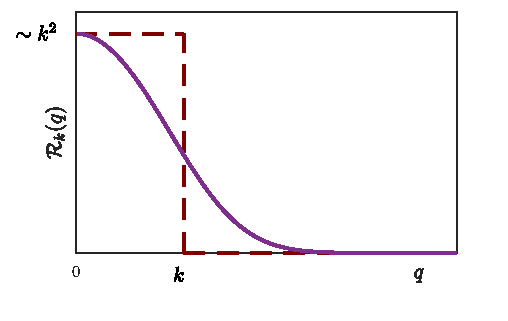
\includegraphics[width=0.95\columnwidth]{Reg.pdf}
\end{center}
\caption{Allure du régulateur choisi pour une valeur de $k$ donnée avec une décroissance exponentielle (ligne continue bleue - c.f. \refeq{RegExp}) et avec une fonction de Heaviside (pointillés rouges -c.f. \refeq{RegHeav}). Ainsi ici nous avons approximativement intégrés les degrés de libertés dans $\simeq [k,\Lambda]$ sans toucher aux autres. On remarque la décroissance douce vers 0 contrairement au régulateur }
\end{figure}

\vspace*{11pt}
\subsubsection{Potentiels et distinction de phase}

En réalité, ce n'est pas vraiment à $\Zc$ que nous allons nous intéresser, mais plutôt aux potentiels qui en dérive, car ils contiennent toutes les informations dont nous avons besoin. 	On reprend alors les différentes définitions données dans la section ... que l'on adapte ici pour prendre en compte la présence du régulateur dans le cas de le limite thermodynamique $\Omega \gg 1/\Lambda^d$. Tout d'abord, pour $k$ fixé on définit une énergie libre 
\begin{equation}
	  W_k[\hv] = \text{ln}{\(\Zc_k[\hv]\)}
\end{equation}
Et de même pour le tenseur des fonctions de corrélation, avec les mêmes notations qu'en ...
\begin{equation}
  G^{(n)}_{k,\{i_j\}} [\{\rv_{j}\} ; \hv] = \derd{^n W_k[\hv]}{h_{i_1}(\rv_1) ... \delta h_{i_n}(\rv_n)}
\end{equation}
En revanche, on ne définit plus exactement la fonctionnelle $\Gamma$ de la même façon, on ne réalise plus vraiment exactement une transformée de Legendre, mais
\begin{equation}
  \Gamma_k [\phiv] = - W_k[\hv] + \int_{\rv} \hv \phiv - \Delta S_k[\phiv],
\end{equation}
Avec $\phiv$ défini comme 
\begin{equation}
  \phiv[\rv, \hv] = \left< \varphiv(\rv) \right> = \derd{W_k[\hv]}{\hv(\rv)}
\end{equation}
Parce que l'on fait une pseudo transformée de Legendre et non pas une vraie, on conserve de cette manière la relation importante :
\begin{equation}
  G^{(2)}_{k, i_1 i_2}[\rv_{i_1}, \rv_{i_2} ; \hv] = \(\Gamma^{(2)}_{k, i_1 i_2}[\rv_{i_1}, \rv_{i_2}, \phiv]\)^{-1}  
\end{equation}
En outre on peut grâce à cela aussi définir, pour $\phiv$ uniforme, le potentiel effectif $V_k$ par
\begin{equation}
	V_k(\phi) = {\left. \frac{1}{|\Omega|} \Gamma_k[\phiv] \right|}_{\phi \text{ unif.}}
\end{equation}
A $k$ fixé, comme introduit dans la section ... à condition de bien réaliser l'adimensionnement, nous pouvons considérer que notre système initial est en fait décrit par un nouveau système fictif dont l'hamiltonien est 
\begin{equation}
	H_k[\varphiv]  = S_k[\varphiv] + \Delta S_k[\varphiv] - \int_\rv \hv \varphiv
\end{equation} 

\commentout{
Remarquons tout de même qu'alors que dans le RG on part du vrai hamiltonien du système originel et on crée à partir de son expression une suite d'hamiltonien associés à des systèmes fictifs, ici on part d'un hamiltonien d'un système fictif en $k = \Lambda$ pour calculer le vrai hamiltonien en $k\to 0$ du vrai système.
De plus nous avons aussi déjà mentionné que c'est la position du minimum du potentiel qui permet de savoir dans quelle phase se trouve le système. Ainsi deux valeurs de $k$ différentes donnent deux systèmes fictifs différents qui peuvent avoir une phase différente. On devra donc chercher en tâtonnant quels sera la température à introduire dans le hamiltonien fictif à $k=\Lambda$ pour obtenir un système vrai à $k \to 0$ qui soit à la transition de phase. On rappelle aussi qu'en $k=\Lambda$ nous partons d'un système fictif "aux fluctuations gelées". Faire évoluer $k$ intègre, i.e. prend en compte, au fur et à mesure de plus en plus les fluctuations du champ décrivant le système. Ceci a pour effet de faire augmenter la température critique
\footnote{En effet on peut comprendre cela en se disant que les fluctuations du champs ont tendance à désordonner le système. Or la "quantité de désordre" permet de définir la phase du système (on pourra penser à de l'eau solide - faible désordre des molécules - et de l'eau liquide -grand désordre -) et ce qui permet "d'obtenir du désordre" dans un système c'est, dans les grandes lignes, la température qu'on lui impose (ce qui explique que jouer sur la température permet de changer de phase de manière générale). Ainsi un système dans lequel on prend en compte les fluctuations aura besoin d'une température moins élevé qu'un système dans lequel on ne les prend pas en compte pour obtenir le même degré de désordre. Ainsi la température pour lequel le désordre sera celui de la transition de phase, i.e. la température critique, sera plus faible} du système fictif. 
On peut donc en conclure que les systèmes fictifs verrons une décroissance de leur température critique et qu'il faudra qu'ils partent de la phase haute température pour avoir une chance de déboucher en $k\to 0$ sur le vrai système exactement à la transition de phase. Un point important est que si le système fictif est dans la phase basse température pour $k\neq 0$ alors le système vrai en $k \to 0$ est aussi dans la phase basse température. Ainsi remarquons que $V_k$ pour $k \neq 0$ est une fonction qui doit être concave autour de l'origine pour assurer l'unicité de son minimum et la convexité de $W_k$ lorsque ce minimum est différent de $0$ et que l'on est dans la phase haute température. Ainsi c'est en observant le caractère concave ou convexe de $V_k$ dans un voisinage de $0$ que l'on peut déterminer la phase du système fictif défini à $k$. 

\begin{figure}[H]
\begin{center}
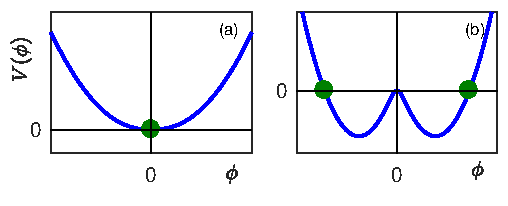
\includegraphics[width=0.95\columnwidth]{CourbePot2.pdf}
\caption{Allure du potentiel. La position de $\phiv_0$ est symbolisée par les points verts. Dans le cas (a), nous sommes dans la phase dite haute température. Dans le cas (b) le potentiel est toujours une fonction convexe mais elle est extra plate autour de l'origine. En physique on dira que le minimum de V ne se trouve pas vraiment en $0$ mais sur les bords de la région plate, suivant certains critères. Remarquons qu'il s'agit bien alors de fonctions concaves et paires.}
\end{center}
\end{figure}
\vspace*{-11pt}

}

\subsubsection{Equation de flot}

On peut alors utiliser toutes les définitions que l'on vient de poser pour extraire l'équation fondamentale du NPRG que l'on appelle l'équation de flot exacte. Il s'agit d'une équation valable pour $k \in ]0, \Lambda]$ décrivant l'évolution de $\Gamma$ avec $k$ lorsqu'on le fait évoluer de $\Lambda$ à $0$. 
\begin{equation}
\partial_t \Gamma_{k}	[\phiv] = \frac{1}{2} \int_\qv \partial_t \Rc_k(\qv) \, G^{(2)}_{k, ij}[\qv, -\qv, \phiv] \, ,
\end{equation}
où $t$ est le temps de RG, défini par $t = \ln(k/\Lambda)$. Avec $G^{(2)}_{k, ij}[\qv, -\qv, \phiv]$ la transformée de Fourier du tenseur $G_k^{(2)}$ définie en \refann{}. 
\begin{equation}
G^{(2)}_{k, ij}[\qv, -\qv, \phiv] = {\(\Gamma^{(2)}_{k, ij}[\qv, -\qv, \phiv]  + \Rc_k(\qv) \)}^{-1}
\end{equation}
En outre, nous avons aussi une condition initiale pour $\Gamma$ puisque d'après les équations \refeq{} il vient
\begin{equation}
	\Gamma_\Lambda [\phiv] = \Gamma_\Lambda 	[\varphiv_0] = S[\varphiv_0]
\end{equation}
Avec $\varphiv_0$ défini comme en \refeq{}.\\

Rappelons que la connaissance de $\Gamma$ permet de connaitre les exposants critiques $\eta$ et $\nu$, cette équation est donc fondamentale. Ainsi, nous avons une équation différentielle avec une condition initiale connue.

Notons que l'intégrale dans cette équation de flot est en fait tronquée par la fonction $q \to \partial_t\Rc_k(q)$ qui pour un $k$ fixé limite, par ses propriétés, l'intervalle d'intégration qui n'est donc jamais véritablement faite sur un domaine infini et peut sans problème être réalisé numériquement.\\


Cependant on peut remarquer que pour connaitre $\partial_t \Gamma$ dans cette équation il nous faut connaitre la dérivée seconde $\Gamma^{(2)}$. Puis si on voulait connaitre $\Gamma^{(2)}$ il nous faudrait connaitre $\Gamma^{(3)}$ et $\Gamma^{(4)}$, ainsi de suite. On dit alors que l'équation est ouverte et n'est donc pas soluble telle quelle. Ce pourquoi nous allons utiliser l'approximation BMW. 




\subsubsection{Approximation BMW} 
 
Le principe de l'approximation BMW \cite{Blaizot} est de considérer que certaines impulsions dans l'expressions des $\Gamma^{(n)}$ ne jouent pas le même rôle que les autres. En effet 

On obtient finalement le système d'équation suivant 
\begin{equation}
\begin{split}
	\partial_t \Gamma_{k, ij}^{(2)}(\pv, \phiv) = & J_3(\pv, \phiv) {\( \partial_\phi \Gamma_{k, ij}^{(2)}(\pv, \phiv) \)}^2 \\
	& - \frac{1}{2}  I_2(\phiv) \, \partial_\phi^{2} \Gamma_{k, ij}^{(2)}(\pv, \phiv)
\end{split}
\end{equation}

\vspace*{11pt}
\subsubsection{La dimension anormale}

Avant de s'occuper de l'application des équations BMW à un modèle concret introduisons le concept de dimension anormale. En effet nous avons mentionner que la fonction de corrélation à deux points évolue, à la transition de phase, schématiquement en $G^{(2)}(r) \sim |r|^{2-d-\eta}$ pour $r \to \infty$. Or cette grandeur $\eta$, qui est un exposant critique, possède aussi le nom de dimension anormale car elle viole à priori la dimension que devrait avoir $G^{(2)}(r)$ d'une longueur à la puissance $2-d$. Pour la prendre en compte dans les équations cela ne découle donc pas naturellement des équations déjà écrite. Pour cela on remarque que cette évolution de $G^{(2)}$ implique aussi $\Gamma^{(2)} \sim \pv^{2-\eta}$ quand $\pv \to 0$. On introduit alors $Z_k$ une grandeur dimensionnée telle que
\begin{equation}
	Z_k = {\left. \frac{\partial \Gamma_k^{(2)}[\pv, \phiv]}{\partial \pv^2} \right|}_{\phiv \text{ unif.} = \phiv_0, \pv = \pv_0 }
\end{equation}

Où $\phi_0$ et $\pv_0$ sont des valeurs arbitraire du champ uniforme et de l'implusion. De cette manière  quand $k \to 0$ nous avons $Z_k \propto \pv^\eta$.
On introduit alors $\eta_k$ tel que
\begin{equation}
	\eta_k = -k \partial_k \ln(Z_k)
\end{equation}

Ainsi nous dirons que $\Gamma^{(2)}_k$ n'a pas vraiment la dimension de $\pv^2$ mais la dimension de $Z_k\pv^2$. Et il a été prouvée\cite{} que ce faisant 
\begin{equation}
 	\lim\limits_{k \to 0} \eta_k  = \eta
 \end{equation}
Ceci est d'une très grande importance pour l'adimensionnement des équations qui est nécessaire pour trouver les points fixes du RG (c.f. \ref{}). Mais de plus c'est cette grandeur qui va nous donner l'exposant critique $\eta$ que l'on recherche.
\vfill
\pagebreak
 
\section{Le modèle continu $O(N)$}

\subsection{Théorie $\varphiv^4$ et modèle $O(N)$}

\subsubsection{Modèle $O(N)$}
On dit qu'un modèle est $O(N)$ si jamais le système est invariant par l'action du groupe de rotation $O(N)$ sur ces degrés de libertés. Plus précisément, soit $J \in O(N)$, et on note $J.V$ l'action de $J$ sur un vecteur $V$ de $\R^N$. Le modèle est dit $O(N)$ si 
\begin{equation}
	H[J \varphiv] = H[\varphiv]	
\end{equation}

Dans la suite nous utiliserons alors une autre grandeurs scalaire invariante sous $O(N)$ pour caractériser les champs uniformes 
\begin{equation}
	\rho = \frac{1}{2}  \phiv^2  
\end{equation}
Ainsi le potentiel effectif $V_k$, $\Gamma^{(2)}$ ou leurs dérivées ne dépendrons plus que de $\rho$ qui est une grandeur scalaire et non plus du vecteur $phiv$.

\subsubsection{Théorie $\varphiv^4$}

Il a été montré \cite{Bellac2012} que lorsque l'on cherche à déterminer les exposants critiques, et que l'on s'intéresse uniquement à ce qu'il peut se passer au voisinage de la température critique alors il suffit d'étudier les premiers ordres du hamiltonien autour de $\varphiv \sim 0$, qui, pour respecter les symétries, dans le modèle $O(N)$ à nécessairement la forme 
\begin{equation}
		H[\varphiv] = \int_\rv \, \left\{ \frac{1}{2}(\nabla \varphiv)^2 + \frac{1}{2}r_0 \varphiv^2 + \frac{u_0}{4!}{\({\varphiv}^{2}\)}^{2} \right\}
\end{equation}

Avec $u_0$ et $r_0$ deux réels. 
C'est donc ce hamiltonien qui est injectée dans les équations du RG permettant d'obtenir les équations de flot et les équations BMW qui nous ont intéressées. Toutes les équations d'un tel système ont été développées, par exemple, dans \cite{benitez2012nonperturbative}. 


\vspace*{11pt}
\subsection{Les équations dans le cas $O(1) \simeq \mathbb{Z}_2$}

Nous écrivons ici ce que donne les équations dans le cas particulier $O(1)$ et nous laissons le cas général en annexe par soucis de concision. Le problème numérique à résoudre est donc : \\

\noindent
{\itshape Trouver $\tY_k(\trho, \tp)$ et $\tW_k(\trho)$ tels que pour tout $k \in [1, 0[$,  $\trho \in [0, +\infty[$ et $\tp \in [0, +\infty[$,}
\begin{align}
	\partial_t \tY_k & = 
	\begin{aligned}[t]
			& \eta_k(1+\tY_k) + \tp \, \partial_{\tp} \tY_k -(2-d-\eta_k)\trho \,\partial_{\trho} \tY_k  \quad  \\
			& \quad + 2\trho \tp^{-2} \left[ {\( \tp^2 \partial_{\trho} \tY_k + \tilde{u}_k\)}^2\, \tJ_3 - \tilde{u}_k^2\ \tI_3 \right] \\
			& \quad - \tI_2 \(  \partial_{\trho} \tY_k / 2 + \trho \,  \partial_{\trho}^2 \tY_k \)
	\end{aligned}
	\label{eqn}\\
	\partial_t \tW_k & = 
	\begin{aligned}[t]
		& (\eta_k-2) \tW_k  + (d-2+\eta_k) \trho \,\partial_{\trho}\tW_k + \frac{1}{2} \partial_{\trho} \tI_1
	\end{aligned}
\end{align}

Avec les notations définies en annexe \refann{}.
Et les conditions initiales
\begin{equation}
	\tY_1(\trho, \tp) = 0 \quad  \text{et} \quad \tW_1(\trho) = r_0' + u_0'\trho
\end{equation}
où $r_0'$ et $u_0'$ viennent de $r_0$ et $u_0$ (c.f. \refeq{}). 
Pour résoudre ce système il manque cependant encore une équation sur $\eta_k$ découlant de la définition même de $Z_k$ en \refeq{} et écrite en annexe.
Ces équations sont dites adimensionnée car nous y avons réalisé l'adimensionnement du RG décrit en section \refsec{} ; ce pourquoi on retrouve un tilde sur toutes les grandeurs qui sont toutes définies dans \cite{}.\\

Ainsi le but est de chercher "un point fixe" en faisant varier $r_0'$ pour se rapprocher de la température critique et du potentiel du système à la température critique. On teste donc plusieurs $r_0'$ avec une dichotomie pour 


\vspace*{11pt}



\section{Méthodes numériques pour la résolution de ces équations}

\subsection{Travail réalisé sur ces équations}




La première partie de notre travail a été de reprendre le développement de ces équations et nous avons réécrit de façon plus modulable et structurée en C++ un code de résolution qui avait déjà été écrit au laboratoire (c.f. \refig{org}). Pour résoudre ces équations de très nombreuses méthodes numériques ont été mises en place, comme des méthodes galerkin \cite{shen1994efficient, LeonardThesis} pour la représentation des fonctions, de simpsons pour le calcul des intégrales, de Runge-Kutta pour la discrétisation temporelle etc., avant qu'un algorithme fonctionnant dans les cas $N=1$ et $d=2$ puisse être trouvé. Cependant, cet algorithme échoue lorsque l'on essaie de l'utiliser en $N \ge 2$ en $d=2$. Nous avons donc essayer d'en comprendre la cause, notamment en réalisant des calculs en des dimensions $d \in [2,3]$ et en les comparants à d'autres codes plus simples que nous avons réécrit, provenant d'autres approximations que BMW. 


\end{multicols}
\begin{figure}[H]
	\begin{center}
		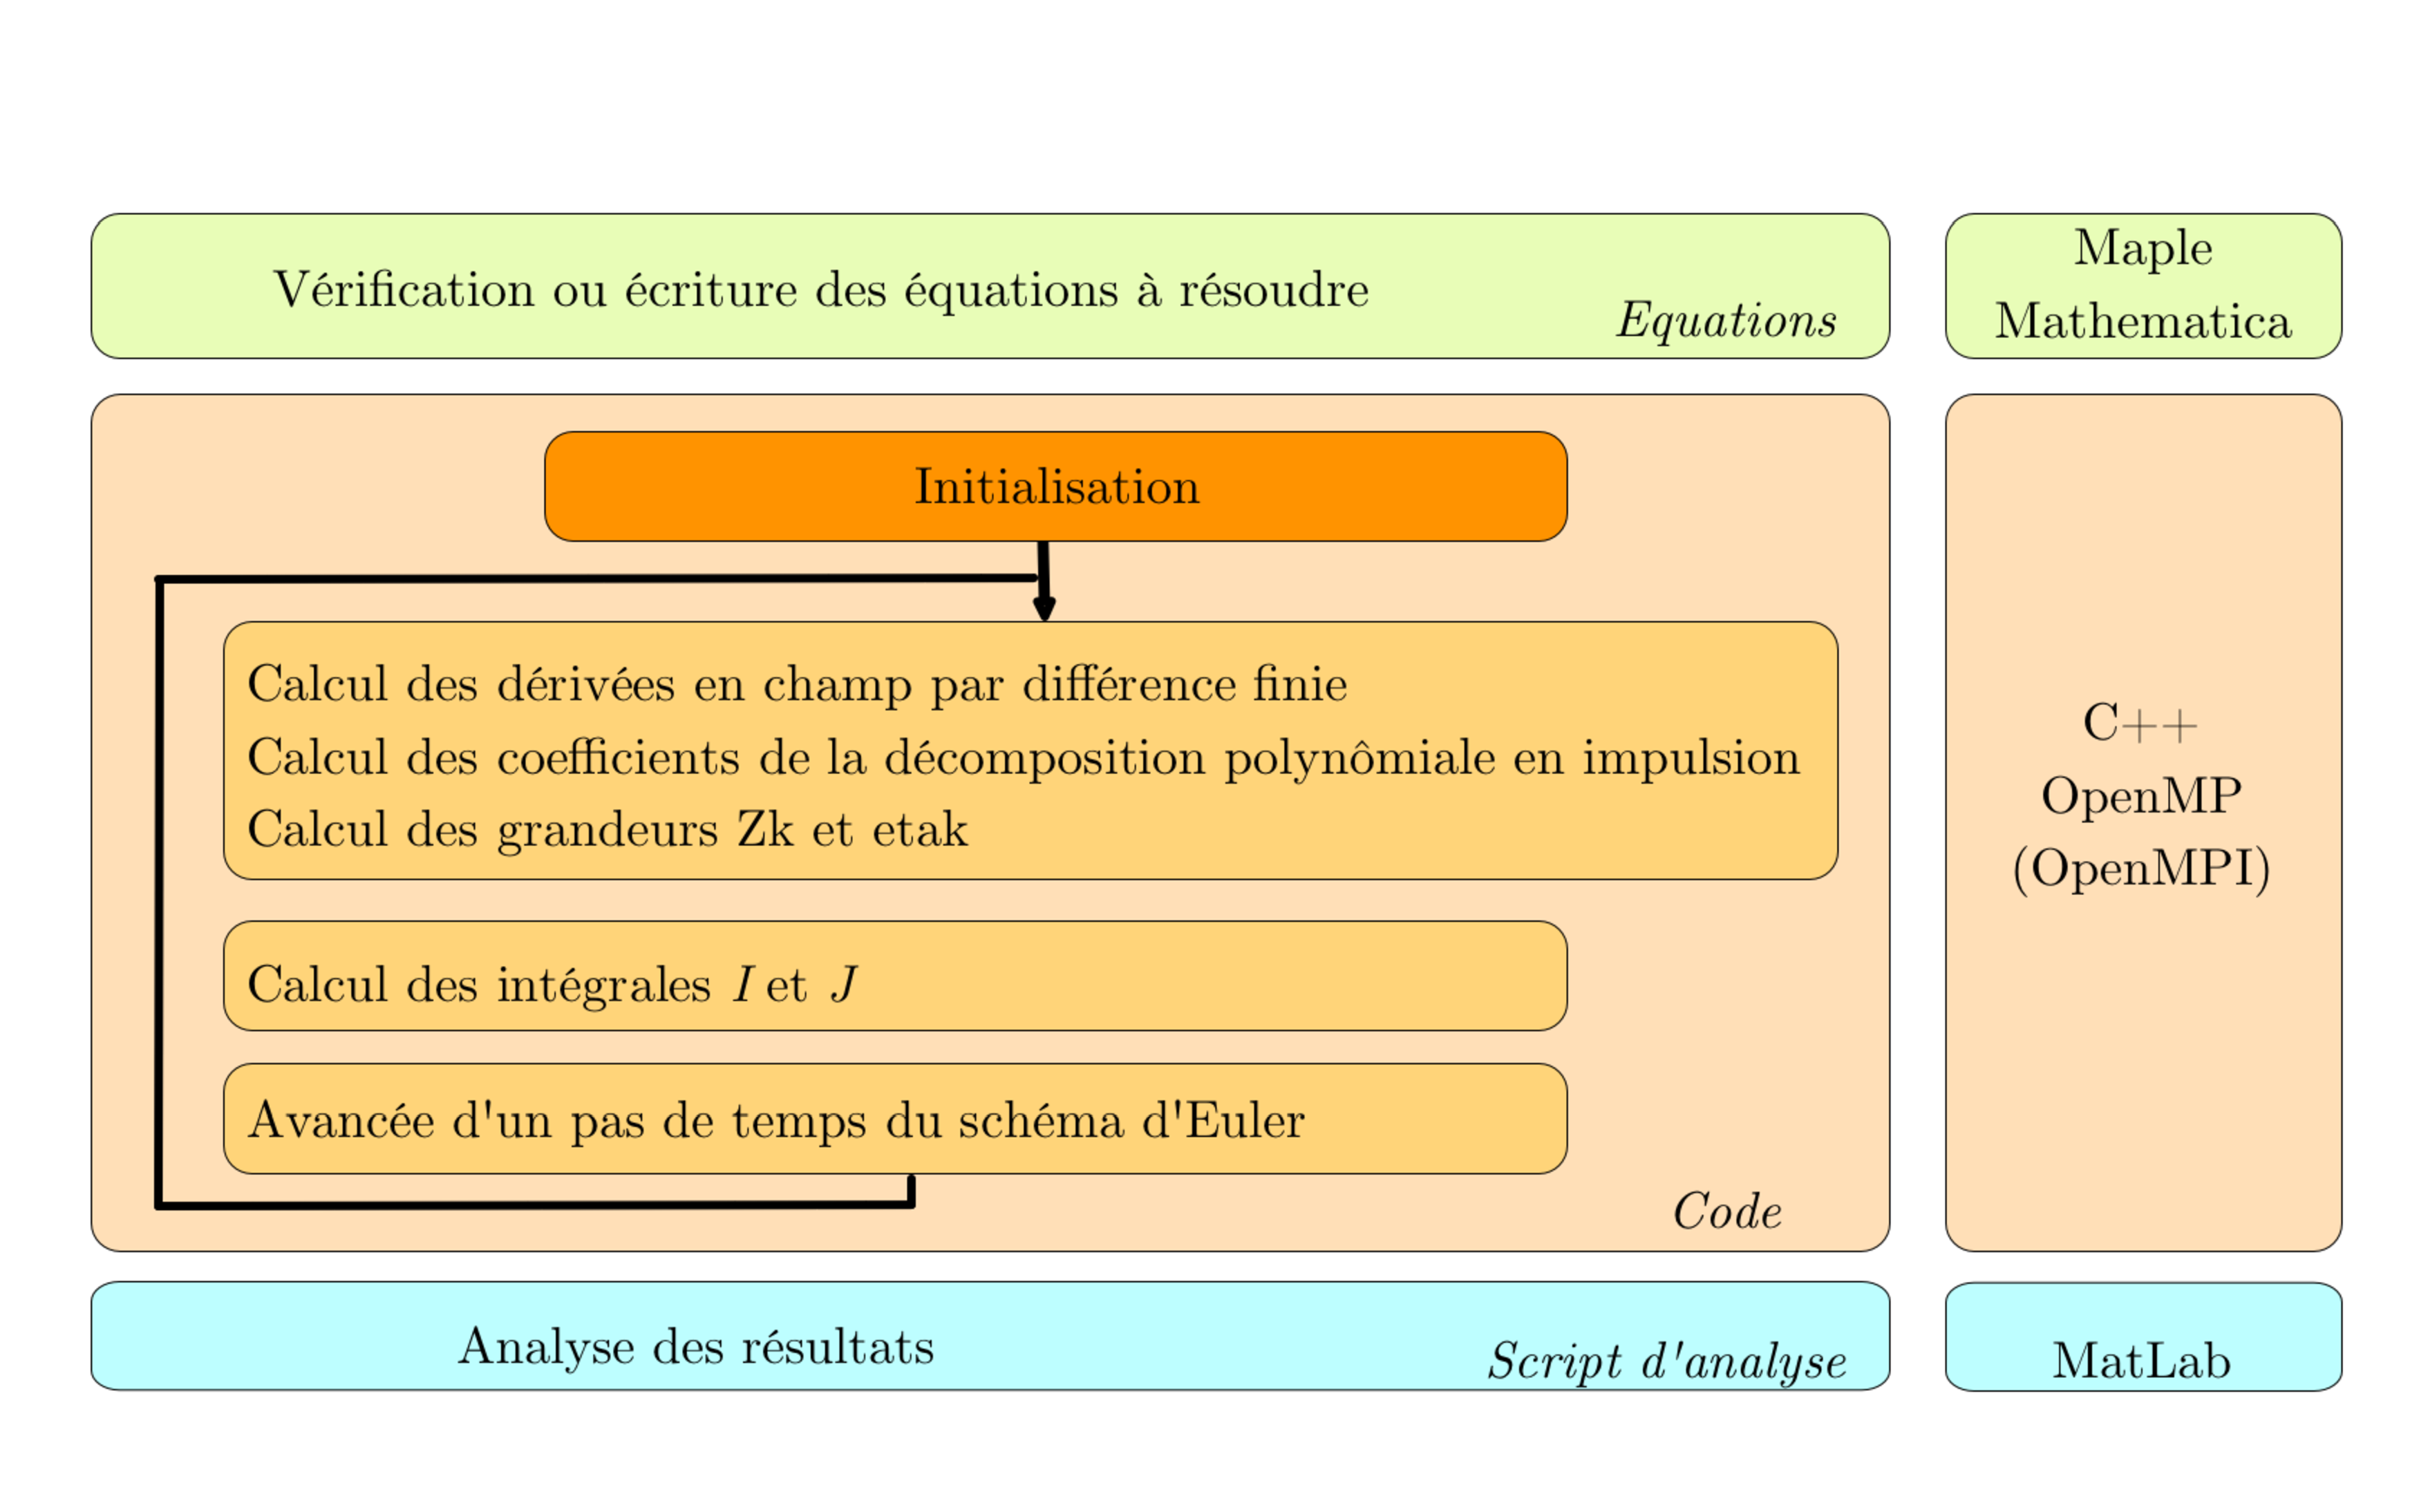
\includegraphics[width=0.95\columnwidth]{Diagramme_Code_2.pdf}
		\caption{Schéma de la répartition du travail effectué. Nous avons commencé par retrouver ou écrire les équations BMW à résoudre (vert). Ensuite nous avons réécrit ou écrit les codes C++ de simulation de ces équations ayant la structure indiquée (rouge). Toutes les parties orangées sont parallélisée sous OpenMP. Enfin nous étudions les résultats à l'aides de scripts Matlab.}
		\label{fig:org}
	\end{center}
\end{figure}

\begin{multicols}{2}


\subsection{Structure de l'algorithme}

Nous avons a résoudre ici un système d'équations intégro-différentielle non linéaires couplées et sans conditions au bords. Pour cela nous utilisons différentes techniques numériques. 

Pour la discrétisation en temps, nous sommes dans l'obligation d'utiliser un schéma explicite à cause de la structure complexe des termes de gauches des équations. Il a été montré qu'un schéma d'Euler explicite d'un pas de temps est suffisant pour obtenir une résolution stable, c'est donc ce qui est utilisé. 

Ensuite nous allons différencier la dépendance en champs (i.e. en $\rho$) à celle en impulsion (i.e. $p$) des fonctions inconnues. Pour ce qui est de la dépendance en champ, il suffit de prendre une grille fixe régulièrement espacé de points. Les dérivées selon cette variable se calculent alors par des schémas de différences finies d'ordre 5. 

Enfin pour la dépendance en impulsion c'est plus compliqué car il faut à la fois pouvoir facilement dériver selon $p$, mais aussi intégrer des expressions qui dépendent des fonctions inconnues - afin d'obtenir les intégrales $I$ et $J$. Au premières versions de ce code, la discrétisation se faisait aussi sur une grille fixe de points régulièrement espacés et les intégrales étaient calculées par des méthodes de Simpsons. Cependant cela c'est avéré ne pas être assez précis dans certaines configurations, les algorithmes n'étaient pas robustes. Pour palier à ce problème c'est une décomposition pseudo spectrale qui a été mise en place à l'aide de décomposition en série sur des polynômes de Tchebytchev associé à une intégration de Gauss-Legendre. 




\subsection{Discrétisation en champ}

Comme nous l'avons mentionné la discrétisation en champ se fait sur une grille fixe de points régulièrement espacés. Les dérivées sont calculées sur 5 points avec des schémas différences finis (\refann{}). Ce choix sur 5 points  a été fait pour essayer de calculer des dérivées le plus précisément possible. Le problème venant des points des bords de la grille de discrétisation, puisque ne possédant pas de condition de bords, nous utilisons des schémas complètements décentrés pour ne faire un calcul que sur les points connus dans la grille. Il s'avère que cette technique reste stable (nous verrons en \refsec{} que cela nous a quand même posé des problèmes pour le modèle d'Ising en deux dimensions). 

Nous avons remarqué aussi que l'on retrouve l'équivalent d'une condition CFL pour le choix du pas de discrétisation $\delta \rho$. En effet le rapport $\delta t / \delta\rho$ doit rester inférieur à une certaine valeur pour conserver la stabilité du schéma.

Enfin il pourrait sembler étranger d'utiliser une discrétisation en champ d'ordre 5 couplée à une discrétisation temporelle d'ordre 1. Cependant l'implémentation d'un schéma de Runge-Kutta a été testé sans pour autant permettre un calcul avec plus de précision ou une plus grande rapidité. 

\subsection{Discrétisation en impulsion}
\subsubsection{Interpolation de Tchbytchev}

Pour la discrétisation en impulsion 


\subsubsection{Calcul de l'interpolé - méthode de Clenshaw}


Afin de calculer la fonction aux points d'interpolation lorsque cela est nécessaire nous utilisons une méthode un peu plus astucieuse que celle consistant à calculer directement la somme de la série.

\begin{proposition}{Algorithme de Clenshaw}.
Soit, de manière générale, une suite de polynômes $\{\Pc_n\}_{n \in \N}$ liés par la relation
\begin{equation}
  \forall x \in \R \quad \Pc_{n+1}(x) = u_n(x)\Pc_n(x) + v_n(x)\Pc_{n-1}(x)
\end{equation}
On souhaite calculer, pour $x \in \R$ donné, 
\begin{equation}
  S = \sum_{l=0}^{N} a_l \Pc_l(x)
\end{equation}
On considère l'algorithme suivant :
\vspace*{-11pt}
\begin{algorithm}[H]
  \begin{algorithmic}[1]
    \STATE $b_{N+2} = 0$ ; $b_{N+1} = 0$
    \FOR{ $m = N .. 1$  }
    \STATE $b_m = a_m + u_m(x)b_{m+1} + v_{m+1}(x)b_{m+2}$
    \ENDFOR
    \STATE $S_1 = a_0\Pc_0(x) + b_1\Pc_1(x) + b_2v_1(x)\Pc_0(x)$
  \end{algorithmic}
\end{algorithm}
\vspace*{-11pt}
\noindent
Alors nous avons $S = S_1$. 
\end{proposition}

\begin{proof}
Ce résultat ce démontre par récurrence sur $m \in \bbrac{1,N}$ en remarquant que,
\begin{equation}
S_1 = S_m +  b_{m+1}\Pc_{m+1}(x) + b_{m+2}v_{m+1}(x)\Pc_{m+2}(x)
\end{equation}
Avec la notation $S_m = \sum\limits_{l=0}^{m} a_l \Pc_l(x)$.
\end{proof}




\subsection{Parallélisation}


Le code a été écrit de manière à rendre sa parallélisation très simple. En effet pour chaque point de la grille en champ on a une fonction discrétisé en impulsion qui est complètement indépendante des autres à l'exception du moment ou l'on calcule les dérivées par rapport à $\rho$. Ainsi il suffit de réaliser l'ensemble des calculs dans des boucles parcourant l'ensemble quasi-indépendant des points de la grille en champs. En utilisant une architecture à mémoire partagée comme openMP on la parallélisation de toutes les parties vertes de \refig{} se fait tout naturellement à l'aide de quelques instructions seulement. 



\pagebreak
\section{Le modèle d'Ising en dimension 2}

On considère le modèle d'Ising classique sur un réseau hypercubique de dimension $d$ (nous avons uniquement travaillé numériquement dans le cas $d=2$ mais nous exposons le formalisme pour une dimension $d$ quelconque). Les longueurs sont exprimées en unité du pas du réseau. On note $\{\ev_\nu\}_{\nu\in\bbrac{1,d}}$ la base cartésienne associée. L'hamiltonien du système est alors donné par
\begin{equation}
H = -J\beta \sum_{\left<\rv, \rv'\right>}S_\rv S_{\rv'}
\end{equation}

Où $S_\rv$ représente la valeur du spin (i.e. sa direction selon l'axe $z$, c.f. \refig{schemaIsing}) à la position $\rv$, comprise dans $\{-1,1\}$. La notation $\left<\rv, \rv'\right>$ signifie que le terme $S_\rv S_{\rv'}$ contribue à la somme si et seulement si ce sont deux spins plus proches voisins du réseau (i.e s'il existe $\nu \in \bbrac{1,d}$ tel que $\rv' = \rv \pm \ev_\nu$). 
\setlength{\unitlength}{1cm}
\begin{figure}[H]
\begin{center}
\begin{picture}(6,3.8)

\put(-0.5,1){\vector(0,1){2}}
\put(-0.8,2){$z$}

\color{cyan}
\put(0,0){\line(1,3){1.2}}
\put(1,0){\line(1,3){1.2}}
\put(2,0){\line(1,3){1.2}}
\put(3,0){\line(1,3){1.2}}
\put(4,0){\line(1,3){1.2}}
\put(5,0){\line(1,3){1.2}}

\put(-0.25,0.45){\line(1,0){5.7}}
\put(0.05,1.25){\line(1,0){5.7}}
\put(0.25,2.0){\line(1,0){5.7}}
\put(0.45,2.70){\line(1,0){5.7}}
\put(0.65,3.35){\line(1,0){5.7}}
\color{red}
\linethickness{0.35mm}

\put(0.15,0.85){\vector(0,-1){0.8}}
\put(1.15,0.05){\vector(0,1){0.8}}
\put(2.15,0.85){\vector(0,-1){0.8}}
\put(3.15,0.05){\vector(0,1){0.8}}
\put(4.15,0.05){\vector(0,1){0.8}}
\put(5.15,0.85){\vector(0,-1){0.8}}

\put(0.4167,1.6){\vector(0,-1){0.7}}
\put(1.4167,0.9){\vector(0,1){0.7}}
\put(2.4167,0.9){\vector(0,1){0.7}}
\put(3.4167,0.9){\vector(0,1){0.7}}
\put(4.4167,1.6){\vector(0,-1){0.7}}
\put(5.4167,0.9){\vector(0,1){0.7}}

\put(0.667,1.7){\vector(0,1){0.6}}
\put(1.667,1.7){\vector(0,1){0.6}}
\put(2.667,2.3){\vector(0,-1){0.6}}
\put(3.667,1.7){\vector(0,1){0.6}}
\put(4.667,1.7){\vector(0,1){0.6}}
\put(5.667,1.7){\vector(0,1){0.6}}

\put(0.9,2.45){\vector(0,1){0.5}}
\put(1.9,2.95){\vector(0,-1){0.5}}
\put(2.9,2.45){\vector(0,1){0.5}}
\put(3.9,2.45){\vector(0,1){0.5}}
\put(4.9,2.95){\vector(0,-1){0.5}}
\put(5.9,2.45){\vector(0,1){0.5}}

\put(1.1167,3.55){\vector(0,-1){0.4}}
\put(2.1167,3.15){\vector(0,1){0.4}}
\put(3.1167,3.15){\vector(0,1){0.4}}
\put(4.1167,3.55){\vector(0,-1){0.4}}
\put(5.1167,3.55){\vector(0,-1){0.4}}
\put(6.1167,3.15){\vector(0,1){0.4}}



\end{picture}
\end{center}
\caption{Exemple de réseau d'Ising en dimension $d=2$. On traite dans le modèle d'Ising des spins avec une seule composante, ce sont donc des vecteurs dont seule la direction peut changer mais pas l'orientation qui est fixé ici selon $z$, perpendiculairement au plan). Le système est dans la phase haute température ($T>T_c$) car les spins ont des directions aléatoire. Ici le nombre de spins représenté est faible, mais comme nous ferons une étude à la limite thermodynamique il est bien plus élevé dans le système étudié.}
	\label{fig:schemaIsing}
\end{figure}

Sur un tel système nous observons une transition de phase du second ordre. En effet il existe une phase (dite de symétrie brisée, ou encore basse température) dans laquelle les spins tendent tous à s'aligner dans une direction privilégiée lorsque la température et faible et que les fluctuations thermiques ne jouent pas un rôle important. Lorsque l'on dépasse la température critique $T_c$ les spins vont avoir une direction plus ou moins aléatoire le système est alors dans une nouvelle phase (dite symétrique). C'est ce modèle qui explique la perte d'aimantation d'un métal à haute température que nous avions mentionné dans l'introduction. \\

La particularité de ce modèle est aussi qu'il a déjà été complètement résolu analytiquement par Onsager \cite{Onsager} en 1944. Tout est donc déjà connu et notamment la température critique de la transition de phase. Avec l'approche BMW nous avons essayé de la retrouver pour valider la qualité de l'approximation et la possibilité de calculer la température critique $T_c$ par le NPRG. \\

Si l'on change l'axe $z$ en $-z$ alors l'hamltonien du système ne change pas. Ainsi ce système possède une symétrie $O(1) \simeq \mathbb{Z}_2$. Il est donc possible de calculer ces exposants critiques en utilisant les équations BMW de la \refsec{} développée avec l'hamiltonien la théorie $\varphiv^4$. La température critique n'étant pas une quantité universelle, elle dépend entièrement du système et prendre un hamiltonien tronqué ne suffit pas, la forme même du réseau est importante. Ce pourquoi nous allons réexprimer le hamiltonien exact complet \refeq{} afin de l'exprimer sous forme de champ et de pouvoir lui appliquer le NPRG. 
\vspace*{11pt} 

\subsection{Modélisation du problème avec des champs}

Pour des raisons pratiques on définit maintenant un hamiltonien légèrement modifié
\begin{align}
  H_\mu &= -J\beta \sum_{\left<\rv, \rv'\right>}S_\rv S_{\rv'} - \mu \beta N_S \\
  H_\mu  &= -J\beta \sum_{\left<\rv, \rv'\right>}S_\rv S_{\rv'} - \mu \beta \sum_\rv S_\rv^2 
\end{align}
Où $N_S$ est le nombre total de spins. Physiquement cela ne change rien car cela ne fait que décaler l'origine des énergies. En revanche cela a un avantage mathématique. En effet, on pose $A_{\rv, \rv'}^{(\mu)}$ la matrice définie implicitement dans $\mathscr{M}_{N_S}(\R)$ par
\begin{equation}
  H_\mu  = -\frac{1}{2} \sum_{\rv, \rv'} S_\rv A_{\rv, \rv'}^{(\mu)}S_{\rv'}
\end{equation}

Il est alors possible de choisir $\mu$ suffisamment grand pour que $A_{\rv, \rv'}^{(\mu)}$ soit à diagonale strictement dominante et donc inversible. Il suffit de prendre $\mu > dJ$. \\

On peut alors réaliser une transformée de Hubbard-Stratanovitch. Pour cela commençons par écrire la fonction de partition du système modèle
\begin{equation}
  \Zc = \sum_{\{S_\rv\}} e^{-H_{\mu}} =\sum_{\{S_\rv\}}  \exp\(\frac{1}{2} \sum_{\rv, \rv'} S_\rv A_{\rv, \rv'}^{(\mu)}S_{\rv'}\)
\end{equation}

Par integration gaussienne \textit{inverse} il vient, 

\begin{equation}
\begin{split}
  \Zc & \propto \sum_{\{S_\rv\}} \int_\R \prod_{\rv} \, \dd \varphi_\rv \, e^{ -\frac{1}{2} \sum\limits_{\rv, \rv'} \varphi_\rv {(A_{\rv, \rv'}^{(\mu)})}^{-1} \varphi_{\rv'} +\sum\limits_\rv  \varphi_\rv S_\rv  } \\
  \Zc & \propto \int_\R \prod_{\rv} \, \dd \varphi_\rv \, e^{ -\frac{1}{2} \sum\limits_{\rv, \rv'} \varphi_\rv {(A_{\rv, \rv'}^{(\mu)})}^{-1} \varphi_{\rv'} + \sum\limits_\rv \ln\(\cosh(\varphi_\rv)\) } \\
\end{split}
\end{equation}

Cependant nous ne pouvons pas exprimer facilement ${(A_{\rv, \rv'}^{(\mu)})}^{-1}$ et pour cela il est pratique de réaliser une Transformée de Tourier Semi-Discrète  \refann{} en posant, pour $\qv \in [-\pi, \pi]^d$,
\begin{equation}
  \hat{\varphi}(\qv) = \sum_\rv \varphi_\rv e^{-i\qv\rv} \quad \text{et} \quad \varphi_\rv = \int_\qv \hat{\varphi}(\qv)  e^{i\qv\rv}
\end{equation}
Il vient alors
\begin{equation}
\begin{split}
  H_\mu = -J\beta & \sum_{\left<\rv, \rv'\right>} \iint_{\qv,\qv'} \hat{\varphi}(\qv) \hat{\varphi}(\qv')  e^{i(\qv\rv+\qv'\rv')} \\
   -\mu\beta & \sum_\rv \iint_{\qv,\qv'} \hat{\varphi}(\qv) \hat{\varphi}(\qv')  e^{i(\qv+\qv')\rv}
\end{split}
\end{equation}
\commentout{
\begin{equation}
\begin{split}
  H_\mu = -J\beta & \sum_{\rv}\sum_{\nu}   \iint_{\qv,\qv'} \hat{\varphi}(\qv) \hat{\varphi}(\qv')  e^{i((\qv+\qv')\rv \pm \qv'\ev_\nu)} \\
   -\mu\beta & \sum_\rv \iint_{\qv,\qv'} \hat{\varphi}(\qv) \hat{\varphi}(\qv')  e^{i(\qv+\qv')\rv}
\end{split}
\end{equation}
\begin{equation}
\begin{split}
  H_\mu = -J\beta & \iint_{\qv,\qv'} \hat{\varphi}(\qv) \hat{\varphi}(\qv')  \sum_{\rv}  e^{i(\qv+\qv')\rv} \sum_{\nu} e^{ \pm i \qv'\ev_\nu}  \\
   -\mu\beta & \sum_\rv \iint_{\qv,\qv'} \hat{\varphi}(\qv) \hat{\varphi}(\qv')  e^{i(\qv+\qv')\rv}
\end{split}
\end{equation}
}
Notons donc simplement
\begin{equation}
  \lambda_\mu(\qv) = -\beta \left\{ J\sum_{\nu} e^{ \pm i \qv \, \ev_\nu} +\mu \right\} 
\end{equation}
Ainsi, il vient, 
\begin{equation}
  H_\mu =   \iint_{\qv,\qv'} \hat{\varphi}(\qv) \hat{\varphi}(\qv')   \lambda_\mu(\qv')   \sum_{\rv}  e^{i(\qv+\qv')\rv} \\
\end{equation}
\begin{equation}
  H_\mu =   \iint_{\qv,\qv'} \hat{\varphi}(\qv) \hat{\varphi}(\qv')   \lambda_\mu(\qv')   D_{N_S}(\qv+\qv') \\
\end{equation}
En définissant le noyaux de Dirichlet $D_{N_S}$ par
\begin{equation}
  \forall \pv \in [-\pi, \pi]^2 \quad D_{N_S} (\pv) =  \sum_{\rv} e^{i \pv \rv} 
\end{equation}
\commentout{
\begin{equation}
  \begin{split}
  \sum_{x=0}^{N_x} e^{ix(\qv+\qv')_x }  = \frac{1 - e^{i(N_x+1)(\qv+\qv')_x}}{1-e^{i(\qv+\qv')_x }} \\
  = \frac{\sin{\(  \frac{(N_x+1)}{2}(\qv+\qv')_x \)}}{\sin{\( \frac{1}{2}(\qv+\qv')_x \) }} e^{i\frac{N_x}{2}(\qv+\qv')_x }
\end{split}
\end{equation}}

\commentout{
On note $\Dc = \Dc([-\pi, \pi]^2)$, soit $f \in \mathcal{D}$, $D_{N_S}$ étant une fonction de $L^2([-\pi, \pi]^2)$, il appartient à $\Dc'$. On montre alors que \cite{}
\begin{equation}
  \lim\limits_{N_S \rightarrow +\infty} \left< D_{N_S} , f \right>_{\Dc', \Dc} =  \left< \delta , f \right>_{\Dc', \Dc}
\end{equation}
}

Ainsi, en prenant la limite $N_S \rightarrow + \infty$ et en raisonnant au sens des distributions, par les propriétés du noyau de Dirichlet, il vient formellement
\begin{equation}
 \lim_{N_S \rightarrow + \infty} H_\mu = - \int_\qv \hat{\varphi}(\qv)  \lambda_\mu(\qv) \hat{\varphi}(-\qv)
\end{equation}
Dans la suite nous ferons l'hypothèse de la limite thermodynamique, selon laquelle $N_S$ est suffisamment grand pour que l'on écrive, par abus de notation, $H_\mu = \lim\limits_{N_S \rightarrow + \infty} H_\mu$. \\
Nous obtenons alors
\begin{equation}
  H_\mu = - \int_\qv \hat{\varphi}(\qv)  \lambda_{\mu}(\qv) \hat{\varphi}(-\qv)
\end{equation}
Et on en déduit la transformée de Fourier de $A_{\rv, \rv'}^{(\mu)}$
\begin{align}
  \hat{A}(\qv, \qv') = 
  \begin{cases}
    \lambda_{\mu}(\qv) \quad  & \text{si } \qv' = - \qv\\
    0 \quad & \text{si } \qv' \neq - \qv
  \end{cases}
\end{align}

Autrement dit, $\hat{A}$ est un operateur diagonal et bien inversible si $\mu > Jd$. Notons,
\begin{equation}
	\gamma(\qv ) = \frac{1}{d} \sum\limits_{\nu=1}^{d} \cos(q_\nu)
\end{equation}
Ainsi l'expression de $\lambda_mu$ se trouve être 
\begin{equation}
	 \lambda_\mu(\qv) = 2\beta\(J d \gamma(\qv) + \mu\)
\end{equation}

En écrivant alors la conservation du produit scalaire de $\ell^2$ dans $L^2(\R)$ opérée par la transformation de Fourier semi-discrète,
\begin{equation}
  \Zc  \propto \int_\R \prod_{\rv} \, \dd \varphi_\rv \, e^{-S_\mu[\varphi] }
\end{equation}
Avec l'action $S$ s'écrivant :
\begin{equation}
  S_\mu[\varphi] = \frac{1}{2} \int_\qv \varphi(\qv) \frac{1}{\lambda_\mu(\qv)} \varphi(-\qv) - \sum\limits_\rv \ln\(\cosh(\varphi_\rv)\)
\end{equation}
Par isometrie de la transformation de Fourier, et donc par le théorème de Parseval, nous réecrivons $S$ sous la forme 
\begin{equation}
  \begin{split}
    S_\mu[\varphi] & = \frac{1}{2} \int_\qv \varphi(\qv) \[\frac{1}{\lambda_\mu(\qv)} - \frac{1}{\lambda_\mu(0)}\] \varphi(-\qv) \\
    &+ \sum\limits_\rv \[\frac{1}{2\lambda_\mu(0)}\varphi_\rv^2 - \ln\(\cosh(\varphi_\rv)\) \]
  \end{split}
\end{equation}
Enfin, soit $\delta \in \R^+_*$, on pose le changement de variable, 
\begin{equation}
  \varphi \rightarrow \delta\sqrt{2 \beta J d} \, \varphi 
\end{equation}
On obtient alors 
\begin{equation}
S_\mu[\varphi] = \frac{1}{2} \int_\qv \hat{\varphi}(\qv)\eo(\qv)\hat{\varphi}(-\qv) + \sum_\rv U(\varphi(\rv))
\end{equation}
Avec, en posant $\tilde{\mu} = \mu/(Jd)$ et $\tilde{\beta} = \beta Jd$,
\begin{equation}
  \eo(\qv) = \delta^2\frac{1 - \gamma(\qv)}{(\gamma(\qv) + \tilde{\mu})(1+\tilde{\mu})}
\end{equation}
\begin{equation}
  U(\phi) = \delta^2 \frac{1}{1+\tilde{\mu}} \frac{1}{2}\phi^2 - \ln\(\cosh\(\delta\sqrt{2\tilde{\beta}}\phi\)\)
\end{equation}

On se retrouve donc ici avec la formulation d'un problème de théorie des champs que l'on peut résoudre avec le NPRG et notamment avec l'approximation BMW. La seule différence avec tout ce qui a été étudié précédemment c'est qu'ici, par Transformée de Fourier semi-discrète les intégrales sur les impulsions ne sont plus calculées sur un domaine infini mais sur "la première zone de Brillouin", i.e. sur un hypercube de longueur $2\pi$. Toutes les formules vu restent sinon valable en intégrant cet ajustement.\\

 La fonction $U$ représente alors le potentiel du système dans l'approximation de champ moyen. Et ainsi le potentiel $V_k$ des équations BMW prend en $k=\Lambda$ la valeur $V_\Lambda = U$. La fonction $\eo$ s'appelle quant à elle la relation de dispersion.\\
 
 
Remarquons de plus que la fonction $U$ est de classe $\Cc^\infty$ dérivable sur $[0,+\infty[$. Ainsi il vient 
\begin{equation}
X(\phi) = \partial_\phi^2 U(\phi) = \delta^2 \frac{1}{1+\tilde{\mu}} - 
\end{equation}

Ceci nous permet de récupérer la valeur que l'on aurait trouvé en calculant la température critique $\tilde{T}_c^{\text{MF}} = T_c^{\text{MF}}/(Jd) $ en s'appuyant sur une théorie de champ moyen. En effet, dans une théorie de champ moyen le potentiel du système est directement le potentiel $U$. Or on rappelle que la phase dans laquelle on se trouve dépend du potentiel, de la position de son minimum et de sa forme de manière générale. Nous savons qu'en dessous de la température critique $U$ est une fonction concave au voisinage de $\phi = 0$ et au dessus c'est une fonction convexe. Ainsi, à la transition $X(0) = 0$. Ceci nous donne

\begin{equation}
 \frac{1}{\tilde{T}_c^{\text{MF}}} = \tilde{\beta}_c^{\text{MF}} \simeq \frac{1}{2(1+\tilde{\mu})}
\end{equation}

Cette valeur nous donne déjà une borne supérieure sur la température critique que l'on recherche. En effet, on sait que la vraie température critique sera toujours plus faible que celle obtenue par approximation de champ moyen\footnote{Ceci s'explique en partie "avec les mains". En effet dans une approximation de champ moyen, comme son nom l'indique les fluctuations des degrés de libertés - ici l'orientation des spins - autour s'une position moyenne se trouvent être négligées. Or leur prise en compte pour la résolution complète du modèle implique que pour une même température le système complet est plus désordonné que ce que le calcul champ moyen nous donne. La température critique vraie sera donc plus basse que la température critique champ moyen} : $T_c < T_c^{\text{MF}}$.


\vspace*{11pt}

\vspace*{11pt}
\subsection{Etapes de la résolution numérique}
La résolution numérique du problème s'est déroulée en plusieurs étapes. Tout d'abord nous avons commencé par écrire les équations BMW qui découlent de la forme de l'action précédemment déterminés. Cependant nous sommes passés par plusieurs étapes. En effet, comme nous travaillons sur un réseau, avec des  \\

Tout d'abord, contrairement au modèle O(N), nous avons commencé par écrire les équations BMW sans les adimmensionner. En effet possédant des  \\

Malheureusement, après avoir écrit une première fois les équations selon la variable $\rho$ à cause d'instabilités numériques constatées au voisinage de $\rho = 0$ provenant probablement du calcul numérique instable des dérivées en ces points nous avons du les réecrire  


\subsection{Les différents jeux d'équation}

Comme ce que nous avions fait dans la description du modèle $O(N)$ nous détaillons ici une seule des équations que nous avons cherché à résoudre.

\vspace*{22pt}

\section{Méthodes et outils numériques pour la résolution d'Ising 2D}

Nous allons passé en revu et justifié ici les principales méthodes numériques que nous avons utilisé pour tenter de résoudre les équations. En grande partie nous avons repris ce qui avait déjà été fait pour la résolution du modèle $O(N)$ mais nous les avons adapter pour pouvoir être utiliser au mieux en deux dimensions.


\subsection{Structure du code}



% Mettre un diagramme

\subsection{Interpolation de Tchebytchev}

Afin de pouvoir calculer les intégrales $J$ avec précision apparaissant dans les équations il semble nécessaire d'interpoler la fonction $\Delta_k$ ainsi que ces dérivées dans le plan des impulsions. Pour cela nous réutilisons encore une interpolation de Tchébytchev en dimension 2. 

\subsubsection{Théorème de décomposition}

Nous rappelons ici un théorème justifiant l'utilisation des polynômes de Tchebytchev comme pôlynomes d'interpolation en dimension 2. Ce théorème et sa démonstrations se trouvent dans l'ouvrage \cite{Tchebychev}. 

\begin{theorem}
  Soit $f : [-1,1]^2 \rightarrow \C$ une fonction continue aux variations bornées (comme définies en \cite{Tchebychev}). On suppose que l'une des dérivées partielles de de $f$ existe et est bornée dans $[-1,1]$. Alors la série $f_N$ définie par :
\begin{equation}
f_N(x,y) = \sum_{i=0} ^{N} \sum_{j=0} ^{N} c_{ij} T_i(x)T_j(y)
\end{equation}
converge uniformément vers $f$ quand $N \rightarrow +\infty$.
\end{theorem}

La condition des variations bornées ne peut bien entendu pas être vérifiée sur nos fonctions mais ...

\vspace*{11pt}

\subsubsection{Décomposition méthode 1}

Soit $f$ une fonction de $[0,\pi]^2$ dans $\R$. Dans un premier temps nous avons opté pour un algorithme de recherche direct des coefficients $c_{ij}$ de sa décomposition en série de polynômes de Tchebytchev très inspiré de la méthode 1D. Supposons, en effet, que l'on veuille effectuer une décomposition à l'ordre $N_C -1$ et donc écrire
\begin{equation}
  f(x,y) \simeq \sum_{i=0}^{N_C-1}\sum_{j=0}^{N_C-1} c_{ij} T_i(x)T_j(y)
\end{equation}

Pour trouver la valeur des coefficients de la matrice $((c_{i,j}))_{i,j}$ on prend les ensembles des racines du polynôme de Tchebytchev  de degré $N_C$, $\left\{x_m\right\}_{0\le m \le N_C-1}$ et $\left\{y_n\right\}_{0\le m \le N_C-1}$ et on impose,
\begin{equation}
  f(x_m, y_n) = \sum_{i=0}^{N_C-1}\sum_{j=0}^{N_C-1} c_{ij} T_i(x_m)T_j(y_n)
\end{equation}
En utilisant les relations des polynômes de Tchebytchev on peut alors determiner les coefficients de la matrice $((c_{ij}))_{i,j}$ avec les formules
\begin{equation}
 c_{ij} = \frac{A}{N_C^2} \sum_{m=0}^{Nc-1} \sum_{n=0}^{Nc-1} f(x_m, y_n)T_i(x_m)T_j(y_n)
\end{equation}
\begin{align}
  A = 
  \begin{cases}
    1 \quad \text{si } i = j = 0 \\
    2 \quad \text{si } i = 0 \text{ et } j \neq 0 \\
    2 \quad \text{si } i \neq 0 \text{ et } j = 0 \\
    4 \quad \text{si } i \neq 0 \text{ et } j \neq 0 \\
  \end{cases}
\end{align}

Cette méthode est extrêmement couteuse puisque pour calculer l'ensemble des coefficients de $((c_{ij}))_{i,j}$ cela demande un algorithme de complexité évlouant en $\mathcal{O}(N_c^2)$ et dejà long pour de faibles valeurs de $N_c$. Ce pourquoi, afin d'obtenir de meilleures précisions sur les intégrales calculées tout en conservant un temps de calcul raisonnable nous avons implémenté la deuxième méthode suivante.


\vspace*{11pt}

\subsubsection{Décomposition méthode 2}
En revanche, il existe une méthode plus astucieuse, inspirée de ce qui est mis en place dans le paquet \textit{chebfun} développé par ... qui permet justement de traiter les interpolations de Tchebytchev sous Matlab. Cette méthode est développée en détails dans \cite{TownsendThesis}. 

Au lieu de faire directement une décomposition sur une base tensorielle de polynomes de Chebychev on commence par réaliser une approcximation de rang faible de la fonction que l'on souhaite approximer. Plus précisemment, on considère les ensembles des racines de Tchebytchev $\left\{x_m\right\}_{0\le m \le N_C-1}$ et $\left\{y_n\right\}_{0\le m \le N_C-1}$. Alors on peut former la matrice 
\begin{equation}
	\mat{F} =((f(x_m, y_n ))_{0\le m,n \le N_C-1}
\end{equation}
et faire de cette matrice une approximation de rang faible par élimination Gaussienne.

\begin{algorithm}[H]
  \begin{algorithmic}[1]
    \STATE Initialisation : $\mat{E}^0 = \mat{F}$; $\mat{F}_0 = 0$; $k = 1$;
    \WHILE{ ${\| \mat{E}^k \|}_{\infty} < \varepsilon $ }
    \STATE $(i_k, j_k) =  {\text{argmax}}_{(i,j)} \left\{\left| \mat{E}^{k-1}_{i,j} \right| \right\}$
    \STATE $\mat{C}^k_{j} = \mat{E}^k_{i_k,j}$;  $\mat{R}^k_{i} = \mat{E}^k_{i,j_k}$; $d_k = \mat{E}^k_{i_k,j_k}$
    \STATE $\mat{E}^k_{i,j} = \mat{E}^{k-1}_{i,j} - d_k^{-1}\mat{C}^k_{j}\mat{R}^k_{i}$
    \STATE $\mat{F}^k_{i,j} = \mat{F}^{k-1}_{i,j} + d_k^{-1}\mat{C}^k_{j}\mat{R}^k_{i}$
    \ENDWHILE
  \end{algorithmic}
\end{algorithm}

Notons $Q$ le rang de l'approximation obetnue. On obtient alors une écriture de $f$ sous la forme 
On obtient alors une expression de la forme 
\begin{equation}
\mat{F} \simeq \tilde{\mat{F}} = \sum_{j=1}^Q d_j \mat{C}^j \mat{R}^j
\end{equation}
Comme nous ne conaissons exactement la fonctions $f$ qu'aux points d'interpolation de Chebychev cela revient au même que d'écrire que nou avons décomposé $f$ comme une somme de produits de fonctions à une variable,
\begin{equation}
f(x,y) \simeq \sum_{j=1}^Q d_jc^j(y)r^j(x)
\end{equation}
On peut alors décomposer les fonctions $c_j$ et $r_j$ sur une base de polynômes de Chebychev comme on peut le faire pour toute fonction d'une seule variable. La décomposition est ainsi un une opération de produit tensoriel. \\







\subsection{Le calcul des intégrales} 

Pour calculer numériquement les différentes intégrales nous nous servons des propriétées de symétries des différentes fonctions. En effet pour tout $\rho \in \R^+$ les fonctions $\eo(.,.)$, $\Rc_k(.,.)$, $\Delta_k(.,.,\rho)$, ...


\subsubsection{Le choix de la quadrature}

On interpole les fonctions des polynômes de Tchebytchev et on utilise toujours une méthode pseudo-specrtrale\footnote{c'est à dire que l'on connait à chaque pas de temps la valeur de la fonction au points d'interpolation de Tchebythchev, ainsi que les coefficients de son développement en série de polynômes de Tchebytchev}. Il semble donc naturel de se demander si la quadrature de Gauss-Legendre est vraiment la mieux adaptée. En effet, pour gagner du temps et utiliser directement la connaissance de la fonction aux points d'interpolation nous avons penser au calcul d'intégrale par la \emph{première règle de Fejer} \cite{} qui permet cela.
 
Cependant cette méthode c'est avérée être inéficace puisque il faut de manière générale plus de points pour obtenir la même précision qu'une quadrature de Gauss Legendre. Et de plus, afin d'assurer la compatibilité entre l'interpolation et la quadrature il est nécessaire que les deux se fassent sur le même nombre de point, ce qui est restrictif. 

% Insert image of calculation by these two quadrature  





\subsubsection{Calcul des intégrales $I$}

Soit $f$ une fonction de $[-\pi, \pi] \times [-\pi, \pi]$ à valeurs dans $\R$. On suppose que $f$ est symétrique par rapport à l'axe des $x=0$, à l'axe des $y=0$ et à l'axe $x=y$. Nous cherchons alors une quadrature pour integrer $f$ sur son domaine de définition. Pour commencer, en utilisant les deux premières symétries,
\begin{equation}
\int_{-\pi}^{\pi} \int_{-\pi}^{\pi} f(x,y) \, \dd x \, \dd y = 4 \int_{0}^{\pi}  \int_{0}^{\pi} f(x,y) \, \dd x \, \dd y
\end{equation} 
On peut alors faire le changement de variable affine  $\(\tilde{x}, \tilde{y}\) \rightarrow \(2x/\pi -1, 2y/\pi -1\) $ donnant,  
\begin{equation}
\begin{split} 
  \int_{0}^{\pi}  \int_{0}^{\pi}  f(x,y) \, & \dd x \, \dd y = \\
 \frac{\pi^2}{4} \int_{-1}^{1} & \int_{-1}^{1} f\(\frac{\pi}{2}\(\tilde{x}+1\),\frac{\pi}{2}\(\tilde{y}+1\)\) \, \dd \tilde{x}  \, \dd \tilde{y} 
\end{split}
\end{equation}
Les intégrales sur le carré unité $[-1,1] \times [-1, 1]$ sont alors calculées avec une quadrature \textit{tensorielle} obtenue à partir d'une quadrature 1D. Il vient des considérations précédentes, 
\begin{equation}
\begin{split}
 \int_{-\pi}^{\pi} \int_{-\pi}^{\pi} f(x,y) \,&  \dd x \, \dd y \simeq \\ 
 \pi^2\sum_{i=0}^{N_{GL}} & \sum_{j=0}^{N_{GL}}w_i w_j f(\frac{\pi}{2}\(\xi_i+1\), \frac{\pi}{2}\(\xi_j+1\))
\end{split}
\end{equation}
Où $\{w_i\}_{i \in \bbrac {1, N_{GL}}}$ sont les poids d'intégration 1D et  $\{\xi_i\}_{i \in \bbrac {1, N_{GL}}}$ les poids d'intégration correspondants. Par construction, $((w_i w_j))_{i,j}$ est une matrice symétrique et par symétrie de $f$ par rapport à la première bissectrice nous pouvons alors réduire la double somme par, 
\begin{equation}
\begin{split}
 \int_{-\pi}^{\pi} \int_{-\pi}^{\pi} f(x,y) \,&  \dd x \, \dd y \simeq \\ 
 \pi^2\sum_{i=0}^{N_{GL}} & \sum_{j=0}^{i-1}w_i w_j 2 f(\frac{\pi}{2}\(\xi_i+1\), \frac{\pi}{2}\(\xi_j+1\)) \, + \\
\pi^2\sum_{i=0}^{N_{GL}} & w_i^2f(\frac{\pi}{2}\(\xi_i+1\), \frac{\pi}{2}\(\xi_i+1\))
\end{split}
\end{equation}
Ce qui permet de réduire le temps de calcul en réduisant légèrement la complexité algorithmique.

\vspace*{11pt}




\subsubsection{Calcul des intégrales $J$}

Soit $(a,b) \in [0,\pi]\times [0,\pi]$. Soit maintenant $f$ et $h$ deux fonctions de $\R^2$ dans $\R$ et  $g$ définie sur  $[-\pi, \pi] \times [-\pi, \pi]$ par $g : (x,y) \rightarrow f(x+a, y+b)$. On suppose, comme précédemment, que $f$ et $h$ sont symétriques par rapport à l'axe $x=0$, à l'axe $y=0$ et à l'axe $x=y$. On fait aussi l'hypothèse qu'elles sont $2\pi$ periodiques. Nous cherchons alors une quadrature pour integrer $g\times h$ sur $[-\pi, \pi] \times [-\pi, \pi]$. Pour cela remarquons que
\begin{equation}
\begin{split}
 & \int_{-\pi}^{\pi} \int_{-\pi}^{\pi} g(x,y) h(x,y) \,  \dd x \, \dd y  = \\
 \int_{0}^{\pi} & \int_{0}^{\pi} [f(x+a, y+b) + f(x+a, y-b)] h(x,y) \, \dd x \, \dd y \, + \\ 
\int_{0}^{\pi} & \int_{0}^{\pi} [f(x-a, y+b) + f(x-a, y-b)] h(x,y)  \, \dd x \, \dd y 
\end{split}
\end{equation}
Et on adopte encore une quadrature de Gauss-Legendre.





\subsection{Dérivées numériques}


\subsection{Complexité algorithmique et parallélisation - problème de rapidité} 

Comme pour le modèle continu $O(N)$ il est possible de paralléliser le code en utilisant de l'openMP \cite{} grain fin sur les boucles en champ. En revanche ici notre code, à cause de la quadrature précise que l'on souhaite avoir sur le calcul des intégrales $J$ le temps de calcul se trouve évoluer en $\mathcal{O}( Q_\text{max} \times N_C^3 \times N_{GL}^2)$. Il vient alors 
\begin{figure}[H]
\begin{center}
	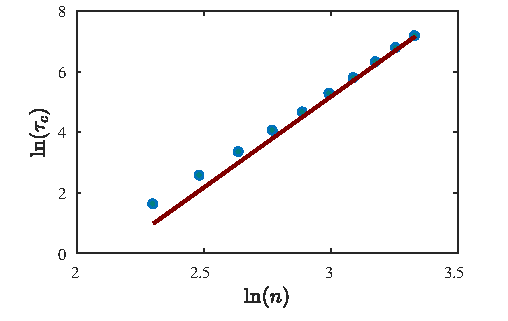
\includegraphics[width=0.95\columnwidth]{ComplexiteTemps.pdf}
\end{center}
\caption{(Points bleus) Logarithme du temps de calcul mesuré $t_c$ de 10 pas de temps du code en fonction du nombre de points d'intégration et d'interpolation. Où l'on a pris $\bar{N} = N_c = N_g$. (Ligne rouge) droite d'équation $y=6x+b$ avec $b$ une constante. Il semble que les points se rapproche du comportement de la droite et ainsi que l'on ait $t_c \propto N^6$. Un interpolation linéaire sur les données dont on dispose donne plus précisément $t_c \propto N^{5,7} $   }
\end{figure}

\pagebreak

\bibliographystyle{plain}
\bibliography{Rapport}


\end{multicols}


\pagebreak

\appendix


\begin{multicols}{2}
\section{Outils pour le développement des équations}


\subsection{Transformée de Fourier}

On rappelle ici les notations utilisée pour définir les transformées de Fourier. Pour cela on considère $\varphiv$ une application de $L^2(\R^d)^N$. On définit alors la transformée de Fourier de $\varphiv$, notée $\hat{\varphiv}$ ou $\text{TF}[\varphiv]$ par, 

\begin{equation}
  \forall \qv \in \R^d \quad \hat{\varphiv}(\qv) = \text{TF}[\varphiv](\qv) = \int_{\R^d} \varphiv(\rv) e^{-i\qv.\rv}\dd \,\rv
\end{equation}
Avec la relation inverse,
\begin{equation}
  \forall \rv \in \R^d \quad \varphiv(\rv)  = \text{TF}^{-1}[\hat{\varphiv}](\rv) = \frac{1}{(2\pi)^d}\int_{\R^d} \hat{\varphiv}(\qv) e^{i\qv.\rv}\dd \,\qv
\end{equation}
On utilise alors la notation plus compacte 
\begin{equation}
  \frac{1}{(2\pi)^d}\int_{\R^d} ... \dd \,\qv \equiv \int_\qv ... \quad \text{et} \quad  \int_{\R^d} ... \dd \,\rv \equiv \int_\rv ... 
\end{equation}

Dans le cas ou l'on a des fonctions définies non pas sur $\R^d$ mais sur un domaine $\Omega \subset \R^d$ fini alors nous aurons les mêmes propriétés avec la relation "d'équivalence"  
\begin{equation}
	 \int_{\qv} ... \overset{\text{$\Omega$ fini}}{\quad \longrightarrow \quad } \frac{1}{\Omega} \sum_{\qv} ...
\end{equation}
Remarquons que lorsque l'on introduit la transformée de Fourier (\refsec{}) pour l'utiliser dans le RG les fonctions $\varphiv$ sont tout d'abord définies sur un ouvert $\Omega$ fini mais par des considérations physique, en passant à "la limite thermodynamique" on en vient à considèrer $\Omega$ comme devenant $\R$ tout entier. En outre, dans le cas où $\varphiv \in \Sr'(\R^d)^N$ (espace des distributions tempérées) on étend la notion de transformée de Fourier $\hat{\varphiv}$ de $\varphiv$ à l'aide du crochet de dualité, 
\begin{equation}
  \forall u \in \Sr(\R^d, \R^N) \quad \left< \hat{\varphiv}, u \right>_{\Sr', \Sr} = \left< \varphiv, \hat{u} \right>_{\Sr', \Sr}
\end{equation}

\vspace*{11pt}



\subsection{Transformée de Fourier Semi Discrète}

Dans le modèle d'Ising à deux dimensions nous introduisons une transformée de Fourier semi discrète car nous travaillons non pas avec des fonctions mais avec des suites. Ainsi soit $\varphi_\rv \in \ell^2$. On peut définir $\hat{\varphi} \in L^2(\R)$ par  
\begin{equation}
  \hat{\varphi}(\qv) = \sum_\rv \varphi_\rv e^{-i\qv\rv}
\end{equation}
  Avec la relation inverse,
\begin{equation}
 \varphi_\rv = \int_{\R^d} \hat{\varphi}(\qv)  e^{i\qv\rv} \dd\, \qv \equiv \int_\qv \hat{\varphi}(\qv)  e^{i\qv\rv}
\end{equation}
On peut de plus démontrer que cette transformation est une isométrie \cite{}.



\vspace*{11pt}
\subsection{Derivation fonctionnelle}

\subsubsection{Définition}
Soit $U$ et $V$ deux espaces de Banach. Soit $F$ une fonctionnelle de $U$ dans $V$. 
Soit $f \in U$. On appelle, si elle existe, dérivée (au sens de Fréchet) de la fonctionelle $F$ prise en $f$, l'application linéaire continu de $\mathcal{L}(U,V)$, notée $D_fF$ telle que, pour $\eps>0$, 
\begin{equation}
\forall h \in U \quad \lim_{ \eps \rightarrow 0 } \frac{\| F[f+\eps h] - F[f] - \eps D_fF.h\|_V}{\eps}  = 0
\end{equation} 
Dans le cas où $U = L^2(\R^d)^N$ et $V = \R$ alors $D_fF \in U'$ (espace des forme linéaires continues de $U$) et on sait qu'il existe, par le théorème de Frechet-Riesz, une quantité unique que l'on note $\delta F[f]/\delta f /in U'(=U)$ telle que 
\begin{equation}
\forall h \in U \quad D_f F.h = {\left< \derd{F[f]}{f}, h \right>}_{U} = \int \derd{F[f]}{f(\rv)} h(\rv) \dd \, \rv	
\end{equation}

\vspace*{11pt}

\subsubsection{Transformée de Fourier d'une dérivée fonctionnelle}

Soit $F$ une fonctionelle de $U = L^2(\R^d)^N$ dans $(\R,|.|)$ et $\varphiv \in U$.
Soit $\rv \in \R^d$.
Alors, 
\begin{equation}
  \derd{F}{\varphiv(\rv)} = \int_{\qv} \derd{F}{\hat{\varphiv}(-\qv)} e^{i\qv.\rv} = \text{TF}^{-1} \left[ \derd{F}{\hat{\varphiv}(-\qv)} \right](\rv) 
\end{equation} 
Et réciproquement nous avons alors aussi, pour $\pv \in \R^d$,  
\begin{equation}
  \derd{F}{\hat{\varphiv}(-\pv)} = \int_{\rv} \derd{F}{\varphiv(\rv)} e^{-i\pv.\rv} = \text{TF} \left[ \derd{F}{\varphiv(\rv)} \right](\pv) 
\end{equation} 

\vspace*{11pt}
%\noindent
{\footnotesize 
\noindent
En effet, par la règle de la chaine de la dérivation de Fréchet nous pouvons écrire, 
\begin{equation}
  \forall \hv \in U \quad D_{\varphiv} F. \hv = D_{\hat{\varphiv}} F. D_{\varphiv} \hat{\varphiv}.\hv 
\end{equation}
Cependant, $\hat{\varphiv}$ est une fonctionnelle de $\varphiv$ (par définition de la TF) de $U$ dans $U$ qui est linéaire en $\varphiv$. Soit $\eps >0$, 
\begin{equation}
  \forall \hv \in U \quad \hat{\varphiv}[\varphiv + \eps \hv] - \hat{\varphiv}[\varphiv] = \eps \hat{\hv} 
\end{equation} 
Il vient directement, par définition de la dérivation au sens de Frechet, $D_{\varphiv} \hat{\varphiv} .\hv = \hat{\hv}$.  
Ainsi,  $D_{\varphiv} F .\hv = D_{\hat{\varphiv}}F.\hat{\hv}$.  On peut alors écrire, 
\begin{align}
  \forall \hv \in U  \quad D_{\varphiv} F .\hv & = \int_{\qv} \derd{F}{\varphiv(\qv)} \int_{\rv} \hv(\rv) e^{-i\qv.\rv} \\
  \forall \hv \in U  \quad D_{\varphiv} F .\hv & = \int_{\rv} \int_{\qv} \derd{F}{\varphiv(\qv)} e^{-i\qv.\rv } \hv(\rv)
\end{align}
}



\subsection{Opérateurs à noyaux}

Nous détaillons dans cette sections quelques propriétés élémentaires des opérateurs à noyaux. Pour plus de détails on pourra regarder \cite{}. Ceci permet de comprendre quelques unes des étapes dans la détermination des équations de flot et BMW. \\



\subsubsection{Définition}

On appelle $S$ un operateur a noyaux, une application de $(L^2(\R^d))^N$, telle que pour tout $(i,j) \in \bbrac{1,N}^2$, il existe une application $A_{i,j} \in L^2(\R^d\times\R^d)$ telle que,  pour tout $\varphiv \in (L^2(\R^d)^N$ et $\rv \in \R^d$
 \begin{equation}
  S[\varphiv]_i(\rv) = \int_{\rv'} \sum_{j=1}^{N} A_{i,j}(\rv,\rv')\varphi_j(\rv')
 \end{equation}
 La matrice $A : (\rv,\rv') \rightarrow ((A_{i,j}(\rv,\rv')))_{i,j}$ est appelée noyau de $S$.  On identifiera alors dans les notations $S$ et $A$ indépendamment. Par Cauchy-Schwartz cette définition a bien  un sens. De plus, on peut montrer que $S$ et est un endomorphisme de $(L^2(\R^d)^N$. Pour plus de clarté, nous utiliserons par la suite la notation d'Einstein : on n'écrit plus la somme sur $j$ dans l'expression de $S$, et de manière générale lorsque un indice est répété dans une expression on suppose qu'il est sommé de $1$ à $N$, 
  \begin{equation}
  S[\varphiv]_i(\rv) \equiv \int_{\rv'} A_{i,j}(\rv,\rv')\varphi_j(\rv')
 \end{equation}
 



\vspace*{11pt}

\subsubsection{TF d'un opérateur à noyaux}

Nous avons vu que $S$ définie comme précédemment était un endomorphisme de $(L^2(\R^d)^N$. Ainsi il est possible d'en définir la transformée de Fourier. Introduisons tout d'abord la transformée de Fourier du noyaux, pour $(i,j) \in \bbrac{1,N}^2$ et $(\qv, \qv') \in (\R^d)^2 $
\begin{equation}
	 \hat{A}_{i,j}(\qv, -\qv') = \iint_{\rv,\rv'} A_{i,j}(\rv,\rv')\,e^{-i\qv.\rv} \, e^{-i \qv'.\rv'} 
\end{equation}
Ce qui implique alors 
\begin{equation}
	 \hat{S}[\varphiv]_i(\qv) = \int_{\qv'} \hat{A}_{i,j}(\qv, -\qv') \hat{\varphi}_j(\qv')
\end{equation}



{\footnotesize
\noindent
En effet, ceci ce démontre en développant le calcul de la transformée de Fourier. Soit $\qv \in \R^d$, $i \in \bbrac{1,N}$
\begin{align}
 \hat{S}[\varphiv]_i(\qv)  = & \int_{\rv} \int_{\rv'} A_{i,j}(\rv,\rv')\varphi_j(\rv') e^{-i\qv\rv}  \\
\hat{S}[\varphiv]_i(\qv)  = & \iint_{\rv, \rv'} \int_{\qv'} A_{i,j}(\rv,\rv') \hat{\varphi}_j(\qv') e^{i\qv'\rv'} e^{- i\qv\rv} \\
 \hat{S}[\varphiv]_i(\qv)  = &   \int_{\qv'} \hat{\varphi}_j(\qv') \left\{ \iint_{\rv, \rv'} A_{i,j}(\rv,\rv')  e^{i\qv'\rv'} e^{- i\qv\rv}  \right\}  \\
\hat{S}[\varphiv]_i(\qv) = & \int_{\qv}  \hat{\varphi}_j(\qv') \hat{A}_{i,j}(\qv, -\qv')
\end{align}
}

\vspace*{11pt}

\subsubsection{Composition de deux opérateurs}

Considérons deux opérateurs à noyaux, $S$ et $T$ de noyaux respectifs $A$ et $B$. La composition de ces deux opérateurs est définie, pour $\rv \in \R^d$, par
\begin{equation}
 	S . T [\varphiv]_i (\rv) = \int_{\rv'}  \left\{ \int_{\rv''} A_{i,k}(\rv, \rv'')B_{k,j}(\rv'', \rv') \right\} \varphi_j(\rv')
\end{equation}
On notera alors aussi pour $(\rv, \rv') \in (\R^d)^2 $
\begin{equation}
   (A . B)_{i,j} (\rv, \rv') = \int_{\rv''} A_{i,k}(\rv, \rv'')B_{k,j}(\rv,'' \rv') 
\end{equation}
Par transformée de Fourier, et par un calcul analogue à celui fait pour un simple noyau, il vient, pour $(\qv, \qv') \in (\R^d)^2$,
\begin{equation}
	\widehat{(A . B)}_{i,j}(\qv, \qv') =\int_{\qv''} \hat{A}_{i,k}(\qv, \qv'')\hat{B}_{k,j}(-\qv'', \qv') 
\end{equation}



\vspace*{11pt}

\subsubsection{Trace d'un opérateur à noyau}

On définit la trace d'un opérateur $S$ de noyaux $A$ par
\begin{equation}
  \text{Tr}\, S \equiv \text{Tr} \, A = \int_{\rv} A_{i,i}(\rv,\rv) 
\end{equation}
Nous pouvons alors de manière similaire à ce qui a été fait pour démontrer l'expression de la transformée de Fourier d'un opérateur à noyau, calculer la relation sur la trace de la transformée de Fourier
\begin{equation}
  \text{Tr} \hat{A} =  \int_{\qv} \hat{A}_{i,i}(\qv,-\qv) 
 \end{equation}



\vspace*{11pt}



\subsubsection{Inverse d'un opérateur à noyau}

Soit S un opérateur à noyau de noyaux A. On fait l'hypothèse, sans justifications, que pour les systèmes physiques que l'on étudie il existe une grandeur appelée l'inverse de S, également un opérateur à noyau, endomorphisme de $(L^2(R^d))^N$, notée $S^{-1}$ telle que, pour $i \in \bbrac{1,N}$ et $\varphiv \in (L^2(R^d))^N$, 
\begin{equation}
	\forall \rv \in \R^d \quad S.S^{-1}[\varphiv]_i(\rv) = \varphi_i (\rv)	
\end{equation}

Si $A$ est le noyau de $S$, on note $A^{-1}$ le noyau de $S^{-1}$.
Nous abordons maintenant pour finir les expressions de la dérivation de la transformée de Fourier de ces inverses.

\end{multicols}



\pagebreak


\section{Complement des algorithmes}

\subsection{Formules de dérivation à 5 points}


On suppose que l'on dispose d'une grille fixe à une dimension de points régulièrement espacées d'une distance $h$. Soit $u$ une fonction de classe $\Cc^5$ sur l'intervalle que défini la grille. Soit $j$ un entier tel que le point d'abscisse $x_j = jh$ soit sur la grille. On note $u_j = u(x_j)$. Les schémas centrés et décentrés d'ordre 5 ci-dessous permettent de calculer les dérivées première et seconde de $u$ par différences finies sur l'ensemble de la grille en n'utilisant sans utiliser de conditions aux limites. \\

Schéma centré :
\begin{align*}
  \partial_xu (jh) &= \frac{1}{12h}\(u_{j-2} - 8u_{j-1} + 8u_{j+1} - u_{j+2}\) \\
  \partial_x^2 u (jh) &= \frac{1}{12h^2}\( -u_{j-2} + 16u_{j-1} - 30u_{j+1} -u_{j+2}\)
\end{align*}

Schémas décentrés gauches : 
\begin{align*}
  \partial_xu (jh) &= \frac{1}{12h}\( -25u_{j} + 48u_{j+1} -36u_{j+2} + 16u_{j+3} - 3u_{j+4} \) \\
  \partial_x^2 u (jh) &= \frac{1}{12h^2} \( 35u_{j} -104u_{j+1} + 114u_{j+2} - 56u_{j+3} + 11u_{j+4}\)\\
  \partial_xu (jh) &= \frac{1}{12h}\( -3u_{j-1} - 10u_{j} +18u_{j+1} - 6u_{j+2} + u_{j+3} \) \\
  \partial_x^2 u (jh) &= \frac{1}{12h^2}\( 11u_{j-1} - 20u_{j} + 6u_{j+1} + 4u_{j+2} - u_{j+3} \) \\
\end{align*}

Schémas décentrés droits : 
\begin{align*}
  \partial_xu (jh) &= \frac{1}{12h}\( 25u_{j} - 48u_{j-1} + 36u_{j-2} - 16u_{j-3} + 3u_{j-4} \) \\
  \partial_x^2 u (jh) &= \frac{1}{12h^2} \( 35u_{j} -104u_{j-1} + 114u_{j-2} - 56u_{j-3} + 11u_{j-4}\)\\
  \partial_xu (jh) &= \frac{1}{12h}\( 3u_{j+1} + 10u_{j} - 18u_{j-1} + 6u_{j-2} - u_{j-3} \) \\
  \partial_x^2 u (jh) &= \frac{1}{12h^2}\( 11u_{j-1} - 20u_{j} + 6u_{j+1} + 4u_{j+2} - u_{j+3} \) \\
\end{align*}

\vspace*{11pt}
\subsection{Propriétés élémentaires des polynômes de Tchebytchev}

On rappelle ici quelques propriétés des polynômes de Tchebytchev. Tout d'abord on défini 
\begin{equation}
	T_n : x \rightarrow \cos(n(\arccos(x)) \quad \forall x \in [-1, 1], \quad \forall n \in \N
\end{equation}
La fonction $T_n$ est une fonction polynomiale associée à un polynôme de $\R_n[X]$ alors appelé polynôme de Tchebytchev de première espèce d'ordre $n$. Nous confondrons la fonction polynomiale et le polynôme qui lui est associé. Il est alors possible de montrer la relation de récurrence 
\begin{equation}
	T_n (X) = 2XT_{n}(X) - T_{n-1}(X) \quad \forall n \ge 1
\end{equation}
Avec $T_0(X) = 1$ et $T_1(X) = X$. Le polynôme $T_n$ possède $n$ racines distinctes réelles $\{x_k\}_k$ dans $[-1,1]$, situées 
\begin{equation}
	x_k = \cos\(\frac{\pi(k+1/2)}{n}\) \quad \forall k \in \bbrac{0,n-1}
\end{equation}
Enfin mentionnons que ces polynômes satisfont à une relation d'orthogonalité discrète. Soit $\{x_k\}_{k \in \bbrac{0,n-1}}$ les $n$ racines de $T_n$. Alors nous avons 
\begin{equation}
		\sum\limits_{k=0}^{n-1}T_i(x_k)T_j(x_k) = ...
\end{equation}



\vspace*{11pt}
\subsection{Quadratures pour le calcul des intégrales}

On cherche à exprimer l'intégrale 

\subsubsection{Quadrature de Gauss-Legendre}

\pagebreak


\section{Equations du modèle d'Ising 2D}

\subsection{Introduction}

On part de la fonction de partition 
\begin{equation}
  \Zc  \propto \int_\R \prod_{\rv} \, \dd \varphi_\rv \, e^{-S_\mu[\varphi] } \\
\end{equation}
Avec l'action $S$ s'écrivant :
\begin{equation}
  S_\mu[\varphi] = \frac{1}{2} \int_\qv \varphi(\qv) \frac{1}{\lambda_\mu(\qv)} \varphi(-\qv) - \sum\limits_\rv \ln\(\cosh(\varphi_\rv)\)
\end{equation}
Par le théorème de Parseval, nous réecrivons $S$ sous la forme 
\begin{equation}
  \begin{split}
    S_\mu[\varphi] & = \frac{1}{2} \int_\qv \varphi(\qv) \[\frac{1}{\lambda_\mu(\qv)} - \frac{1}{\lambda_\mu(0)}\] \varphi(-\qv) \\
    &+ \sum\limits_\rv \[\frac{1}{2\lambda_\mu(0)}\varphi_\rv^2 - \ln\(\cosh(\varphi_\rv)\) \]
  \end{split}
\end{equation}
Enfin, soit $\delta \in \R^+_*$, on pose le changement de variable, 
\begin{equation}
  \varphi \rightarrow \delta\sqrt{2 \beta J d} \, \varphi 
\end{equation}
On obtient alors 
\begin{equation}
S_\mu[\varphi] = \frac{1}{2} \int_\qv \hat{\varphi}(\qv)\eo(\qv)\hat{\varphi}(-\qv) + \sum_\rv V_0(\varphi(\rv))
\end{equation}
Avec, en posant $\tilde{\mu} = \mu/(Jd)$ et $\tilde{\beta} = \beta Jd$,
\begin{equation}
  \eo(\qv) = \delta^2\frac{1 - \gamma(\qv)}{(\gamma(\qv) + \tilde{\mu})(1+\tilde{\mu})}
\end{equation}
\begin{equation}
  V_0(\rho) = \delta^2 \frac{1}{1+\tilde{\mu}} \rho - \ln\(\cosh\(2\delta\sqrt{\tilde{\beta}\rho}\)\)
\end{equation}

De plus, on note $\tilde{\beta}_c^{\text{MF}}$ la valeur de $\tilde{\beta}$ en champ moyen à la temperature critique. En faisant un développement limité à l'ordre 1 en $\rho$ nous avons
\begin{equation}
V_0(\rho) = \delta^2\( \frac{1}{1+\tilde{\mu}} - 2\tilde{\beta}\)\rho + \mathcal{O}(\rho^2)
\end{equation}
Ainsi, nous obtenons 
\begin{equation}
\tilde{\beta}_c^{\text{MF}} \simeq \frac{1}{2(1+\tilde{\mu})}
\end{equation}

\vspace*{11pt}



\subsection{Les équations BMW en $\rho$ dimensionnées}

On pose 
\begin{equation}
\Gamma^{(2)}_{k}(p_x, p_y, \rho) = \eo(p_x, p_y) + \Delta_k(p_x, p_y, \rho) + \partial^2_{\phi} V(\phi)
\end{equation}
\begin{equation}
  W(\phi) = \partial_{\phi} V(\phi) \quad \text{et} \quad X(\phi) = \partial^2_{\phi} V(\phi)
\end{equation}
Les équations à résoudre numériquement sont
\begin{equation}
\begin{split}
\partial_t  \Delta_k(p_x, p_y, \rho)  = & - 2\rho I_3(\rho) u_k^2(\rho)  + 2\rho J_3(p_x, p_y, \rho) {\[ u_k(\rho) + \partial_\rho \Delta_k(p_x, p_y, \rho) \]}^{2} \\
& - \frac{1}{2}I_2(\rho)\[\partial_\rho \Delta_k(p_x, p_y, \rho) + 2\rho\partial_\rho^2 \Delta_k(p_x, p_y, \rho) \]
\end{split} 
\end{equation}
\begin{equation}
\partial_t W_k(\rho) = \frac{1}{2} \partial_\rho I_1 (\rho)
\end{equation}
Avec les notations
\begin{equation}
J_n (p_x, p_y, \rho) = \frac{1}{(2\pi)^2} \int_{-\pi}^\pi \int_{-\pi}^\pi \partial_t \Rc_k(q_x, q_y) \,
G_k^{n-1}(q_x,q_y,\rho)G_k(p_x+q_x,p_y+q_y,\rho) \, \dd q_x \,\dd q_y
\end{equation}
\begin{equation}
I_n (\rho) = \frac{1}{(2\pi)^2} \int_{-\pi}^\pi \int_{-\pi}^\pi \partial_t \Rc_k(q_x, q_y) \,
G_k^{n}(q_x,q_y,\rho) \, \dd q_x \,\dd q_y
\end{equation}
\begin{equation}
G_k(q_x,q_y,\rho) = \frac{1}{\eo(q_x, q_y) + \Delta_k(q_x, q_y, \rho) + m^2_k(\rho) + \Rc_k(q_x, q_y) }
\end{equation}
\begin{equation}
\partial_\rho I_n(\rho) = - n \frac{1}{(2\pi)^2} \int_{-\pi}^\pi \int_{-\pi}^\pi \partial_t \Rc_k(q_x, q_y) G_k^{n+1}(q_x,q_y,\rho)\(\partial_\rho \Delta_k(p_x, p_y, \rho) + u_k(\rho) \) \, \dd q_x \,\dd q_y
\end{equation}
\begin{equation}
m_k^2 (\rho) = \partial_\phi^2 V(\phi) = W(\rho) + 2\rho\partial_\rho W(\rho)
\end{equation}
\begin{equation}
u_k(\rho) = \partial_\rho m_k^2(\rho) = 3\partial_\rho W(\rho) + 2\rho\partial_\rho^2 W(\rho)
\end{equation}
On pose la fonction
\begin{equation}
  \tau(q_x, q_y) = \frac{\eo(q_x, q_y)}{2k^2 {\|\eo\|}_{\infty}}
\end{equation}
On choisit alors le régulateur
\begin{equation}
  \Rc_k(q_x, q_y) = \frac{\alpha \eo(q_x, q_y)}{\exp\(2\tau(q_x, q_y)\) -1 }
\end{equation}
\begin{equation}
  \partial_t \Rc_k(q_x, q_y) = \alpha \eo(q_x, q_y) \frac{\tau(q_x, q_y)}{\sinh^2\(\tau(q_x, q_y)\)}
\end{equation}
Et nous pouvons calculer
\begin{equation}
  {\|\eo\|}_{\infty} = \underset{(p_x, p_y) \in [-\pi,\pi]^2}{\text{sup}} \eo(p_x, p_y) = \frac{2\delta^2}{\mu^2 -1}
\end{equation} 


\vspace*{11pt}



\subsection{Les équations BMW en $\phi$}

\subsubsection{Les équations BMW en $\phi$ dimensionnées}

On rappelle les notations : 
\begin{equation}
  W(\phi) = \partial_{\phi} V(\phi) \quad \text{et} \quad X(\phi) = \partial^2_{\phi} V(\phi)
\end{equation}
On doit alors résoudre
\begin{equation}
\begin{split}
\partial_t  \Delta_k (p_x, p_y, \phi) = &  J_3(p_x, p_y, \phi) {\(\partial_\phi \left\{ \Delta_k (p_x, p_y, \phi) + X(\phi) \right\}\)}^2 \\
& - I_3(\phi){(\partial_\phi X(\phi))}^2 - \frac{1}{2} I_2(\phi) \partial_\phi^2 \Delta_k(p_x, p_y, \phi) 
\end{split}
\end{equation}
\begin{equation}
\partial_t X(\phi) = \frac{1}{2} \partial_\phi^2 I_1(\phi)
\end{equation}
On garde ici des expressions similaires pour les intégrales que ce que l'on avait en $\rho$,

\begin{equation}
J_n (p_x, p_y, \phi) = \frac{1}{(2\pi)^2} \int_{-\pi}^\pi \int_{-\pi}^\pi \partial_t \Rc_k(q_x, q_y) \,
G_k^{n-1}(q_x,q_y,\phi)G_k(p_x+q_x,p_y+q_y,\phi) \, \dd q_x \,\dd q_y
\end{equation}
\begin{equation}
I_n (\phi) = \frac{1}{(2\pi)^2} \int_{-\pi}^\pi \int_{-\pi}^\pi \partial_t \Rc_k(q_x, q_y) \,
G_k^{n}(q_x,q_y,\phi) \, \dd q_x \,\dd q_y
\end{equation}
\begin{equation}
G_k(q_x,q_y,\phi) = \frac{1}{\eo(q_x, q_y) + \Delta_k(q_x, q_y, \phi) + X(\phi) + \Rc_k(q_x, q_y) }
\end{equation}
\begin{equation}
\partial_\phi I_n(\phi) = - n \frac{1}{(2\pi)^2} \int_{-\pi}^\pi \int_{-\pi}^\pi \partial_t \Rc_k(q_x, q_y) G_k^{n+1}(q_x,q_y,\phi)\(\partial_\phi \Delta_k(p_x, p_y, \phi) + \partial_\phi X(\phi) \) \, \dd q_x \,\dd q_y
\end{equation}
\begin{equation}
\begin{split}
\partial_\phi^2 I_n(\phi) = & - n \frac{1}{(2\pi)^2} \int_{-\pi}^\pi \int_{-\pi}^\pi \partial_t \Rc_k(q_x, q_y) G_k^{n+1}(q_x,q_y,\phi)\(\partial_\phi^2 \Delta_k(p_x, p_y, \phi) + \partial_\phi^2 X(\phi) \) \, \dd q_x \,\dd q_y \\
& + n(n+1) \frac{1}{(2\pi)^2} \int_{-\pi}^\pi \int_{-\pi}^\pi \partial_t \Rc_k(q_x, q_y) G_k^{n+2}(q_x,q_y,\phi){\(\partial_\phi \Delta_k(p_x, p_y, \phi) + \partial_\phi X(\phi) \)}^2 \, \dd q_x \,\dd q_y
\end{split}
\end{equation}



\vspace*{11pt}

\subsubsection{Les équations BMW en $\phi$ adimensionnées en impulsion}

On note $\tp_x = k^{-1}p_x$ et $\tp_y = k^{-1}p_y$. Ainsi que
\begin{center}
$\bDelta_k(\tp_x, \tp_y,\phi) = \Delta_k(p_x, p_y,\phi)$; $\bJ_n(\tp_x, \tp_y,\phi) = J_n(p_x, p_y,\phi)$ ; $\bRc_k(\tp_x, \tp_y) = \Rc_k(p_x, p_y) $ \\
$\beo(\tp_x, \tp_y) = \eo(p_x, p_y) $ ; $\btau(\tp_x, \tp_y) = \tau(p_x, p_y) = \beo(\tp_x, \tp_y)/(k^2 {\|\eo\|}_{\infty})$ ; $\bpRc(\tq_x, \tq_y) = \partial_t \Rc_k(q_x, q_y) $ \\
\end{center}
Les équations se réécrivent
\begin{equation}
\begin{split}
\partial_t  \bDelta_k (\tp_x, \tp_y, \phi) = & - I_3(\phi){(\partial_\phi X(\phi))}^2 + \bJ_3(\tp_x, \tp_y, \phi) {\(\partial_\phi \left\{ \bDelta_k (\tp_x, \tp_y, \phi) + X(\phi) \right\}\)}^2 \\
& - \frac{1}{2} I_2(\phi) \partial_\phi^2 \bDelta_k(\tp_x, \tp_y, \phi) + \tp_x \partial_{\tp_x}  \bDelta_k + \tp_y \partial_{\tp_y}  \bDelta_k 
\end{split}
\end{equation}
\begin{equation}
\partial_t X(\phi) = \frac{1}{2} \partial_\phi^2 I_1(\phi)
\end{equation}
En effet, l'expression de la nouvelle derivée par rapport au temps est : 
\begin{equation}
  \begin{split}
    \partial_t \Delta_k (p_x, p_y, \phi){|}_{p_x, p_y, \phi} & = \partial_t \bDelta_k (\tp_x, \tp_y, \phi) {|}_{\tp_x, \tp_y, \phi}   + \partial_t \tp_x  {|}_{p_x} \partial_{\tp_x}  \bDelta_k (\tp_x, \tp_y, \phi) + \partial_t \tp_y  {|}_{p_y} \partial_{\tp_y}  \bDelta_k(\tp_x, \tp_y, \phi) \\
    \partial_t \Delta_k (p_x, p_y, \phi){|}_{p_x, p_y, \phi} & = \partial_t \bDelta_k  (\tp_x, \tp_y, \phi){|}_{\tp_x, \tp_y, \phi}  -  \tp_x \partial_{\tp_x}  \bDelta_k (\tp_x, \tp_y, \phi) -  \tp_y \partial_{\tp_y}  \bDelta_k (\tp_x, \tp_y, \phi) 
  \end{split}
\end{equation}
De plus nous avons toujours pour dérivée temporelle du régulateur
\begin{equation}
  \begin{split}
    \bpRc(\tq_x, \tq_y)  =  \alpha \beo \frac{\btau}{\sinh^2(\btau)}
  \end{split}
\end{equation}

\vspace*{11pt}
\noindent
Les intégrales se calculent selon
\begin{equation}
\bJ_n (\tp_x, \tp_y, \phi) = \frac{k^2}{(2\pi)^2}  \int_{-\frac{\pi}{k}}^{\frac{\pi}{k}} \int_{-\frac{\pi}{k}}^{\frac{\pi}{k}}  \bpRc(\tq_x, \tq_y) \,
\bG_k^{n-1}(\tq_x,\tq_y,\phi)\bG_k(\tp_x+\tq_x,\tp_y+\tq_y,\phi) \, \dd \tq_x \,\dd \tq_y
\end{equation}
\begin{equation}
I_n (\phi) = \frac{k^2}{(2\pi)^2} \int_{-\frac{\pi}{k}}^{\frac{\pi}{k}} \int_{-\frac{\pi}{k}}^{\frac{\pi}{k}} \bpRc(\tq_x, \tq_y)  \,
\bG_k^{n}(\tq_x,\tq_y,\phi) \, \dd \tq_x \,\dd \tq_y
\end{equation}
\begin{equation}
\bG_k(\tq_x,\tq_y,\phi) = \frac{1}{\beo(\tq_x, \tq_y) + \bDelta_k(\tq_x, \tq_y, \phi) + X(\phi) + \bRc_k(\tq_x, \tq_y) }
\end{equation}
\begin{equation}
\begin{split}
\partial_\phi^2 I_n(\phi) = & - n \frac{k^2}{(2\pi)^2} \int_{-\frac{\pi}{k}}^{\frac{\pi}{k}} \int_{-\frac{\pi}{k}}^{\frac{\pi}{k}}  \bpRc(\tq_x, \tq_y) \bG_k^{n+1}(\tq_x,\tq_y,\phi)\(\partial_\phi^2 \bDelta_k(\tp_x, \tp_y, \phi) + \partial_\phi^2 X(\phi) \) \, \dd \tq_x \,\dd \tq_y \\
& + n(n+1) \frac{k^2}{(2\pi)^2} \int_{-\frac{\pi}{k}}^{\frac{\pi}{k}} \int_{-\frac{\pi}{k}}^{\frac{\pi}{k}}  \bpRc(\tq_x, \tq_y) \bG_k^{n+2}(\tq_x,\tq_y,\phi){\(\partial_\phi \bDelta_k(\tp_x, \tp_y, \phi) + \partial_\phi X(\phi) \)}^2 \, \dd \tq_x \,\dd \tq_y
\end{split}
\end{equation}


\vspace*{11pt}
\noindent
\textbf{Calcul du $Z_k$}\\

On commence par définir 
\begin{equation}
\eo^0 ={\left. \frac{\partial \eo}{ \partial {{p_x}^2}} \right|}_{p_x = 0, p_y = 0}
\end{equation}
On montre alors en faisant un developpement limité que
\begin{equation}
\eo(\pv)  \underset{\pv = 0}{\sim} \frac{\delta^2}{4\,(1+\mu)^2} \, \pv^2 \quad \text{avec} \quad \pv^2 = p_x^2 + p_y^2
\end{equation}
Pour calculer $Z_k$ on utilise une des définitions équivalentes
\begin{equation}
Z_k = 1+\frac{1}{\eo^0}{\left. \frac{\partial \Delta_k}{\partial {p_x}^2} \right|}_{p_x = 0, p_y = 0, \phi = 0}  \quad \text{et} \quad 
Z_k = 1+\frac{1}{2\eo^0}{\left. \frac{\partial^2 \Delta_k}{\partial {p_x}^2} \right|}_{p_x = 0, p_y = 0, \phi = 0} 
\end{equation}
Ce qui donne en pratique
\begin{equation}
Z_k = 1+\frac{2\,(1+\mu)^2}{\delta^2}{\left. \frac{\partial^2 \Delta_k}{\partial {p_x}^2} \right|}_{p_x = 0, p_y = 0, \phi = 0} = 1+\frac{2\,(1+\mu)^2}{\delta^2\, k^2}{\left. \frac{\partial^2 \bDelta_k}{\partial {\tp_x}^2} \right|}_{p_x = 0, p_y = 0, \phi = 0}
\end{equation}
En outre par définition nous avons aussi
\begin{equation}
\eta_k = -\partial_t \ln Z_k 
\end{equation}

\vspace*{11pt}
\subsubsection{Les équations BMW en $\phi$ totalement adimensionnées}

On note $\tphi = \sqrt{Z_k}\phi$. Etant donnée que l'on effectue le changement à des valeurs de $k$ très faibles ($k \simeq \exp(-3)$), on considèrera que $\beo(\tp_x,\tp_y) \simeq \eo^0\,k^2(\tp_x^2+\tp_y^2)$. On adimensionne aussi les fonctions en plus des variables :

\begin{equation*}
1 + \frac{\bDelta_k(\tp_x, \tp_y,\phi)}{\eo^0 \pv^2} = Z_k(1+\tY_k(\tp_x, \tp_y,\tphi)) \quad \text{et} \quad \tX(\tphi) = \frac{1}{Z_k k^2} X(\phi)
\end{equation*}


\vspace*{11pt}
\noindent
\textbf{Etude des termes en $\bDelta_k(\tp_x, \tp_y,\phi)$} \\

La dérivée de $\bDelta_k$ par rapport à $t$ se réécrit :
\begin{equation}
\begin{split}
\partial_t  \bDelta_k (\tp_x, \tp_y, \phi) {|}_{\tp_x, \tp_y, \phi } = & \partial_t (Z_k(1+\tY_k(\tp_x, \tp_y,\tphi)\eo^0\pv^2  - \eo^0\pv^2 ) {|}_{\tp_x, \tp_y, \tphi} \\ 
& + \partial_t \tphi  {|}_{\phi}\, \partial_{\tphi} (Z_k(1+\tY_k(\tp_x, \tp_y,\tphi)\eo^0 \pv^2 - \eo^0\pv^2 )
\end{split}
\end{equation}
Ceci donne l'expression suivante
\begin{equation}
\begin{split}
\partial_t  \bDelta_k (\tp_x, \tp_y, \phi) {|}_{\tp_x, \tp_y, \phi } = & - \eo^0 \pv^2 \eta_k Z_k (1+\tY_k(\tp_x, \tp_y,\tphi)) + 2 \eo^0 \pv^2 Z_k (1+\tY_k(\tp_x, \tp_y,\tphi)) \\
& - 2 \eo^0 \pv^2  + \eo^0 \pv^2 Z_k \partial_t \tY_k(\tp_x, \tp_y,\tphi) -  \frac{1}{2} \eo^0 \pv^2 \eta_k Z_k \tphi \partial_{\tphi} \tY_k(\tp_x, \tp_y,\tphi) 
\end{split}
\end{equation}
De plus nous avons aussi concernant les dérivées de  $\bDelta_k$
\begin{equation}
\begin{split}
\tp_x \, \partial_{\tp_x}  \bDelta_k (\tp_x, \tp_y, \phi) = 2\eo^0 p_x^2 Z_k (1+\tY_k(\tp_x, \tp_y,\tphi)) + \eo^0 \tpv^2 Z_k \tp_x \partial_{\tp_x} \tY_k(\tp_x, \tp_y,\tphi) - 2 \eo^0 p_x^2 \\ 
\tp_y \, \partial_{\tp_y}  \bDelta_k (\tp_x, \tp_y, \phi) = 2\eo^0 p_y^2 Z_k (1+\tY_k(\tp_x, \tp_y,\tphi)) + \eo^0 \tpv^2 Z_k \tp_y \partial_{\tp_y} \tY_k(\tp_x, \tp_y,\tphi) - 2 \eo^0 p_y^2 
\end{split}
\end{equation}
Et nous en déduisons alors
\begin{equation}
\begin{split}
\tp_x \, \partial_{\tp_x}  \bDelta_k (\tp_x, \tp_y, \phi) + \tp_y \, \partial_{\tp_y}  \bDelta_k (\tp_x, \tp_y, \phi)= & 2\eo^0 \pv^2 Z_k (1+\tY_k(\tp_x, \tp_y,\tphi))  - 2 \eo^0 \pv^2 \\ 
& \eo^0 \tpv^2 Z_k \( \tp_x \partial_{\tp_x} \tY_k(\tp_x, \tp_y,\tphi) + \tp_y \partial_{\tp_y} \tY_k(\tp_x, \tp_y,\tphi) \)
\end{split}
\end{equation}
Ainsi que pour les dérivées par rapport à $\phi$
\begin{equation}
\partial_{\phi}  \bDelta_k (\tp_x, \tp_y, \phi) = \eo^0 \pv^2 Z_k^{\frac{3}{2}} \partial_{\tphi} \tY_k(\tp_x, \tp_y,\tphi) \quad \text{et} \quad  \partial_{\phi}^2 \bDelta_k (\tp_x, \tp_y, \phi) = \eo^0 \pv^2 Z_k^2 \partial_{\tphi} \tY_k(\tp_x, \tp_y,\tphi) 
\end{equation}


\vspace*{11pt}
\noindent
\textbf{Etude des termes en $X(\phi)$} \\

La dérivée de $X$ par rapport à $t$ devient de même que pour $\bDelta$
\begin{equation}
\begin{split}
\partial_t  X(\phi) {|}_{\phi} = & \partial_t (Z_k k^2\tX(\tphi)) {|}_{\tphi} + \partial_t \tphi  {|}_{\phi}\, \partial_{\tphi} (Z_k k^2\tX(\tphi)) \\ 
\partial_t  X(\phi) {|}_{\phi} = & Z_k k^2\partial_t \tX(\tphi) - Z_k k^2 (\eta_k -2)\tX(\tphi) - \frac{1}{2} Z_k k^2  \eta_k\tphi \, \partial_{\tphi}\tX(\tphi)
\end{split}
\end{equation}
Et pour la dérivée en $\phi$ nous avons
\begin{equation}
\partial_{\phi} X(\phi) = k^2 Z_k^{\frac{3}{2}} \partial_{\tphi} \tX(\tphi)
\end{equation}


\vspace*{11pt}
\noindent
\textbf{Adimensionnement du régulateur}\\

On remarque qu'avec l'approximations faite sur $\eo$ le régulateur s'écrit
 \begin{equation*}
\bRc_k(q_x, q_y) = \Rc_k(q) = \alpha \frac{Z_k \eo^0 k^2 q^2}{\exp\(\frac{\eo^0}{ {\|\eo\|}_{\infty} } \, \frac{q^2}{k^2} \) - 1} 
\end{equation*} 
On adimensionne le régulateur en posant
\begin{equation*}
r_k(\tq) = \frac{\bRc_k(\tq_x, \tq_y)}{\eo^0 q^2 Z_k} = \alpha \frac{1}{\exp\(\frac{\eo^0}{ {\|\eo\|}_{\infty} } \, \tq^2 \) - 1} 
\end{equation*} 
Ainsi on en déduit
\begin{equation}
\partial_t \Rc_k(q) {|}_{q} = \partial_t (\eo^0 q^2 Z_k r_k(\tq)) {|}_{\tq} + \partial_t \tq {|}_{q} \, \partial_{\tq} r_k(\tq)
\end{equation}
\begin{equation}
\partial_t \Rc_k(q) {|}_{q} = \eo^0 k^2 Z_k \tq^2 \left\{ -\eta_k r_k(\tq) - \tq \partial_{\tq} r_k(\tq) \right\}
\end{equation}
Avec l'expression 
\begin{equation}
\partial_{\tq} r_k(\tq) = - \alpha \frac{\eo^0}{2 {\|\eo\|}_{\infty} } \tq \frac{1}{\sinh^2\(\frac{\eo^0}{2 {\|\eo\|}_{\infty}} \tq^2 \)}
\end{equation}
Et on remarquera aussi que 
\begin{equation}
\frac{\eo^0}{{\|\eo\|}_{\infty} } = \frac{\mu -1}{8(\mu+1)}
\end{equation}

\vspace*{11pt}
\noindent
\textbf{Adimensionnement des intégrales et leur expression}\\

On adimensionne aussi les intégrales
\begin{equation*}
\tJ_n(\tp_x, \tp_y,\tphi) = \frac{Z_k^{n-1}}{k^{2(2-n)}}\bJ_n(\tp_x, \tp_y,\phi) \quad \text{et} \quad \tI_n(\tphi) = \frac{Z_k^{n-1}}{k^{2(2-n)}}I(\phi)
\end{equation*} 
Et leurs équations deviennent
\begin{equation}
\tJ_n (\tp_x, \tp_y, \tphi) = \frac{1}{(2\pi)^2}  \int_{-\frac{\pi}{k}}^{\frac{\pi}{k}} \int_{-\frac{\pi}{k}}^{\frac{\pi}{k}} \eo^0 \tq^2 \left\{ -\eta_k r_k(\tq) - \tq \partial_{\tq} r_k(\tq) \right\}   \,
\tG_k^{n-1}(\tq_x,\tq_y,\tphi) \tG_k(\tp_x+\tq_x,\tp_y+\tq_y,\tphi) \, \dd \tq_x \,\dd \tq_y
\end{equation}
\begin{equation}
\tI_n (\tphi) = \frac{1}{(2\pi)^2}  \int_{-\frac{\pi}{k}}^{\frac{\pi}{k}} \int_{-\frac{\pi}{k}}^{\frac{\pi}{k}} \eo^0 \tq^2 \left\{ -\eta_k r_k(\tq) - \tq \partial_{\tq} r_k(\tq) \right\}   \,
\tG_k^{n}(\tq_x,\tq_y,\tphi) \, \dd \tq_x \,\dd \tq_y
\end{equation}
\begin{equation}
\tG_k(\tq_x,\tq_y,\phi) = \frac{1}{\eo^0 \tq^2 \left\{  1 + \tY_k(\tq_x, \tq_y, \tphi)  + r_k(\tq) \right\} + \tX(\tphi) }
\end{equation}
\begin{equation}
\begin{split}
\partial_{\tphi}^2 & \tI_n(\tphi) =  - n \frac{1}{(2\pi)^2} \int_{-\frac{\pi}{k}}^{\frac{\pi}{k}} \int_{-\frac{\pi}{k}}^{\frac{\pi}{k}} \eo^0 \tq^2 \left\{ -\eta_k r_k(\tq) - \tq \partial_{\tq} r_k(\tq) \right\}  \tG_k^{n+1}(\tq_x,\tq_y,\tphi)\( \eo^0 \tq^2 \partial_{\tphi}^2 \tY_k(\tp_x, \tp_y, \tphi) + \partial_{\tphi}^2 \tX(\tphi) \) \, \dd \tq_x \,\dd \tq_y \\
& + n(n+1) \frac{1}{(2\pi)^2} \int_{-\frac{\pi}{k}}^{\frac{\pi}{k}} \int_{-\frac{\pi}{k}}^{\frac{\pi}{k}} \eo^0 \tq^2 \left\{ -\eta_k r_k(\tq) - \tq \partial_{\tq} r_k(\tq) \right\}   \tG_k^{n+2}(\tq_x,\tq_y,\tphi){\(\eo^0 \tq^2\partial_{\tphi} \tY_k(\tp_x, \tp_y, \tphi) + \partial_{\tphi}   \tX(\tphi)\)}^2 \, \dd \tq_x \,\dd \tq_y
\end{split}
\end{equation}





\vspace*{11pt}
\noindent
\textbf{Ecriture des équations finales}\\

En rassemblant toute les expressions précédents ceci nous permet d'écrire les équations
\begin{align}
\partial_t \tY(\tp_x, \tp_y,\tphi) & = 
\begin{aligned}[t]
& \eta_k(1+\tY_k(\tp_x, \tp_y,\tphi)) + \frac{1}{2} \eta_k \tphi \partial_{\tphi} \tY_k(\tp_x, \tp_y,\tphi) - \frac{1}{2} \tI_2(\tphi) \partial_{\tphi}^2 \tY_k(\tp_x, \tp_y, \tphi)\\
& \quad + \frac{1}{\eo^0\tpv^2}\left\{ {\( \eo^0\tpv^2 \partial_{\tphi} \tY_k(\tp_x, \tp_y,\tphi) + \partial_{\tphi} \tX(\tphi)\)}^2 \tJ_3(\tp_x, \tp_y,\tphi) - {\( \partial_{\tphi} \tX(\tphi) \)}^2 \tI_3(\tphi)\right\} \\
& \quad + \tp_x \partial_{\tp_x} \tY_k(\tp_x, \tp_y,\tphi) + \tp_y \partial_{\tp_y} \tY_k(\tp_x, \tp_y,\tphi) \\ \\
\end{aligned}
\label{eqn} \\
\partial_t \tX(\tphi) & = 
\begin{aligned}[t]
(\eta_k -2)\tX(\tphi) + \frac{1}{2}\eta_k\tphi \, \partial_{\tphi}\tX(\tphi) + \frac{1}{2} \partial_{\tphi}^2 \tI_1(\tphi)
\end{aligned}
\end{align}
On notera aussi l'équation de flot qui permet de récupérer le potentiel directement donnée par
\begin{equation}
  \partial_t \tV(\tphi) = -2\tV(\tphi) + \frac{1}{2}\eta_k\tphi \partial_{\tphi}\tV(\tphi) + \frac{1}{2}\tI_1(\tphi)  
\end{equation}

\vspace*{11pt}
\noindent
\textbf{Equation sur $\eta_k$} \\

Pour obtenir l'équation sur $\eta_k$ on commence par partir du fait que
\begin{equation}
\lim\limits_{\pv \rightarrow 0} \left\{ 1 +  \frac{\bDelta_k(\tp_x, \tp_y, 0)}{\eo^0 \pv^2} \right\} = 1 + \frac{1}{\eo^0}\frac{\partial  \bDelta_k(\tp_x, \tp_y, 0) }{\partial \pv^2 } = Z_k
\end{equation}
En utilisant la définition de $\tY$ il vient alors le résultat
\begin{equation}
Z_k = Z_k(1 + \tY(0,0,0)) \quad \Leftrightarrow \quad \tY_k(0,0,0) = 0 \quad \forall k
\end{equation}
Or ce résultat nous donne $\partial_t \tY_k(0,0,0) = 0$. Et on en déduit
\begin{equation}
\eta_k = \frac{1}{2} \tI_2(0) \partial_{\tphi}^2 \tY(0,0,0) 
\end{equation}



\vspace*{11pt}
\noindent
\textbf{Les expressions des régulateurs précédents} \\

Afin d'assurer une compatibilité des équations, et comme maintenant il nous faut avec un un régulateur qui est de la même dimension que la dérivée seconde du potentiel il est nécéssaire de changer légèrement l'expression de $\Rc_k$ que l'on a utilise dans les deux premiers étapes du flot. On prend ici
\begin{equation}
\Rc_k(q_x, q_y) = \alpha \frac{Z_k \eo(q_x, q_y)}{\exp(2\tau(q_x, q_y)) -1}
\end{equation}
Ainsi on en déduit directement les formules suivantes
\begin{equation}
\partial_t \Rc_k(q_x, q_y) = \alpha Z_k \frac{\eo(q_x, q_y)}{\sinh(\tau(q_x, q_y)}   \left\{ \frac{\tau(q_x, q_y)}{\sinh(\tau(q_x, q_y))} - \eta_k \frac{1}{2\exp(\tau(q_x, q_y))} \right\}
\end{equation}
\begin{equation}
\bpRc(\tq_x, \tq_y) = \alpha Z_k \frac{\beo(\tq_x, \tq_y)}{\sinh(\btau(\tq_x, \tq_y))}   \left\{ \frac{\btau(\tq_x, \tq_y)}{\sinh(\tau(\tq_x, \tq_y))} - \eta_k \frac{1}{2\exp(\btau(\tq_x, \tq_y))} \right\}
\end{equation}

\commentout{
\begin{equation*}
\tDelta_k(\tp_x, \tp_y,\tphi) = \frac{1}{Z_k k^2} \bDelta_k(\tp_x, \tp_y,\phi) \quad \text{et} \quad \tX(\tphi) = \frac{1}{Z_k k^2} X(\phi)
\end{equation*}
Ainsi que pour les integrales
\begin{equation*}
\tJ_n(\tp_x, \tp_y,\tphi) = \frac{Z_k^{n-1}}{k^{2(2-n)}}\bJ_n(\tp_x, \tp_y,\phi) \quad \text{et} \quad \tI_n(\tphi) = \frac{Z_k^{n-1}}{k^{2(2-n)}}I(\phi)
\end{equation*} 
Il vient alors les équations
\begin{equation}
\begin{split}
\partial_t  \tDelta_k (\tp_x, \tp_y, \tphi) = & (\eta_k -2)\tDelta_k(\tp_x, \tp_y, \tphi) + \frac{1}{2}\eta_k\tphi \, \partial_{\tphi}\tDelta_k(\tp_x, \tp_y, \tphi) \\
& - \tI_3(\tphi){(\partial_\phi \tX(\tphi))}^2 + \tJ_3(\tp_x, \tp_y, \tphi) {\(\partial_{\tphi} \left\{ \tDelta_k (\tp_x, \tp_y, \tphi) + \tX(\tphi) \right\}\)}^2 \\
& - \frac{1}{2} \tI_2(\tphi) \partial_{\tphi}^2 \tDelta_k(\tp_x, \tp_y, \tphi) + \tp_x \partial_{\tp_x}  \tDelta_k(\tp_x, \tp_y, \tphi) + \tp_y \partial_{\tp_y}  \tDelta_k(\tp_x, \tp_y, \tphi) 
\end{split}
\end{equation}
\begin{equation}
\partial_t \tX(\tphi) =  (\eta_k -2)\tX(\tphi) + \frac{1}{2}\eta_k\tphi \, \partial_{\tphi}\tX(\tphi) + \frac{1}{2} \partial_{\tphi}^2 \tI_1(\tphi)
\end{equation}

Avec pour expression des integrales
\begin{equation}
\tJ_n (\tp_x, \tp_y, \phi) = \frac{1}{(2\pi)^2}  \int_{-\frac{\pi}{k}}^{\frac{\pi}{k}} \int_{-\frac{\pi}{k}}^{\frac{\pi}{k}}  \bpRc(\tq_x, \tq_y) \,
\tG_k^{n-1}(\tq_x,\tq_y,\phi)\bG_k(\tp_x+\tq_x,\tp_y+\tq_y,\phi) \, \dd \tq_x \,\dd \tq_y
\end{equation}
}



\end{document}
